\documentclass[11pt,a4paper]{article}

\usepackage[margin=2.3cm]{geometry}
\usepackage{amsmath,amssymb}
\usepackage{graphicx}
\usepackage{booktabs}
\usepackage{xcolor}
\usepackage{enumitem}
\usepackage[hidelinks]{hyperref}
\usepackage{caption}

\emergencystretch=1.5em
\captionsetup{font=small,labelfont=bf,width=.92\textwidth}
\setlength{\parskip}{4pt plus 1pt}
\setlength{\parindent}{0pt}

\newcommand{\code}[1]{\texttt{#1}}
\newcommand{\bst}[1]{\textbf{#1}}
\newcommand{\Kp}{K'}
\newcommand{\TopK}{\operatorname{TopK}}
\newcommand{\PH}[1]{\textcolor{red}{[#1]}}

\title{Top-$(K{+}J)$ with the RBLapSum surrogate versus hard Top-$\Kp$,\\
with the code carried between blocks\\[2pt]
\large Research note: the K+J grid under \code{code\_residual}}
\author{}
\date{2026-10-04.}

\begin{document}
\maketitle
\vspace{-2em}

% ============================================================
\section{Purpose and summary of conclusions}
% ============================================================

The K+J note (\code{docs/kj-vs-hard-topk.tex}) compared, on an 8-layer
TinyStories model with an abs-TopK bottleneck on the residual stream after
every block, the RBLapSum \code{through\_rank\_kappa} surrogate -- $K$ active
features, gradient to a pool of $K+J$ -- with hard Top-$\Kp$ at $\Kp = K+J$.
Its 25 cells were all \emph{stream-carried}: each block re-encodes the
decoded stream it receives. This note repeats the same 25 cells with one
flag changed, \code{activation\_bottleneck.code\_residual = true}: the
$K$-sparse code itself is carried from block to block, and each block adds
its encoded contribution to it instead of re-encoding the stream.

Two questions are asked of the new family, the same two as before -- does
the surrogate with $K$ active features reach hard Top-$\Kp$ at a fixed pool
$\Kp = K+J$, and how much does widening $J$ help at fixed $K$ -- and a third
one across the two families: cell by cell, what does carrying the code
change, for the hard baselines and for the surrogate cells.

The main conclusions are:

\begin{itemize}[leftmargin=1.4em]
\item \textbf{Carrying the code lowers the loss of every hard Top-$\Kp$
baseline by $0.061$--$0.075$ nats}, at all five $\Kp$: a code-carried
Top-$\Kp$ lands at or below the stream-carried Top-$2\Kp$. The best model of
either grid is code-carried hard Top-512 at $1.3622$, against $1.4146$ for the
best stream-carried model (the $(256,256)$ post-norm surrogate cell).

\item \textbf{For the surrogate the carry is nearly neutral.} In the $T=2$
arm the ten cells move by $-0.030$ to $+0.013$ nats (mean $-0.012$): small
gains on the diagonal $J=K$, none at the wide windows of $K=32$. The ordering
in $J$ is unchanged, and widening $J$ still helps monotonically at every $K$.

\item \textbf{The post-norm arm becomes unstable.} Every post-norm cell with
$K \le 128$ shows recurrent gradient-norm spikes, and five of the ten cells
collapse to the unigram level -- $J=K$ at $K = 32, 64, 128$, and $(64,192)$,
$(64,448)$; the five that finish end within $0.04$ nats of their
stream-carried twins. No $T=2$ or hard cell spiked beyond recovery.

\item \textbf{The candidate window no longer substitutes for active
features.} At a fixed pool no code-carried surrogate cell beats hard
Top-$\Kp$: on the diagonal $J=K$, where the stream-carried surrogate won by
$0.009$--$0.014$, it now trails by $0.055$--$0.065$. At a matched active count
the surrogate's margin over hard Top-$K$ shrinks from $0.107 / 0.087 / 0.064
/ 0.041$ (stream carried, $K = 32$ to $256$) to $0.047 / 0.010$ at $K = 32,
64$ and reverses to $-0.021 / -0.032$ at $K = 128, 256$.

\item \textbf{Weakening the surrogate's support term under the carry only
hurts.} At $K=32$, $T=2$, scaling the support term by $\gamma = 0.8$, $0.6$,
$0.4$ costs $0.007$--$0.034$ nats relative to the full code-carried
surrogate, and the first-order scope, which removes the products of support
terms along the carry, costs $0.007$--$0.024$; the penalty grows with $J$.
The compounding of support terms along the carry is therefore not what
limits the code-carried surrogate at $T=2$: the full term with the plain
backward is its best variant at every $J$. \PH{K=64, 128, 256 to follow}
\end{itemize}

% ============================================================
\section{The code residual}
% ============================================================

\paragraph{Notation.}
The model has $L = 8$ blocks of width $d = 768$. Block $l$ contributes
$\Delta_l(x) \in \mathbb{R}^d$ to a stream $x$: the attention output plus the
MLP output, each computed from its pre-norm as in the plain transformer.
Bottleneck $l$ has an encoder $E_l \in \mathbb{R}^{N \times d}$ and a decoder
$D_l \in \mathbb{R}^{d \times N}$ with $N = 1536$, and $\TopK$ denotes the
abs-TopK operation that keeps the $K$ coordinates of largest magnitude and
zeroes the rest. $\mathrm{N}_l$ is the optional RMSNorm on the bottleneck's
output (``post-norm''), or the identity; the last bottleneck never has one,
since the final norm follows it. $x_0$ is the token embedding.

\paragraph{Stream carried (the K+J note).}
With the \code{residual\_out} placement at every block,
\begin{equation}
x_{l+1} \;=\; \mathrm{N}_l\!\Big(D_l \,\TopK\big(E_l\,(x_l + \Delta_l(x_l))\big)\Big),
\qquad l = 0, \dots, L-1,
\label{eq:stream}
\end{equation}
and $x_L$ goes to the final norm and the unembedding. Every stream between
blocks is a decoded $K$-sparse code, but block $l+1$ computes its code from
the decoded stream again: with $c_{l+1} = \TopK(E_l(x_l + \Delta_l))$ the
next code is $\TopK\big(E_{l+1}(\mathrm{N}_l(D_l c_{l+1}) + \Delta_{l+1})\big)$,
and since $E_{l+1} D_l$ is not the identity, a coordinate kept by block $l$
can be dropped by block $l+1$ even when $\Delta_{l+1} = 0$.

\paragraph{Code carried (\code{code\_residual = true}, the definition used here).}
\begin{align}
c_1 &= \TopK\big(E_0\,(x_0 + \Delta_0(x_0))\big), \label{eq:cr0}\\
x_l &= \mathrm{N}_{l-1}(D_{l-1}\, c_l), \qquad
c_{l+1} = \TopK\big(c_l + E_l\,\Delta_l(x_l)\big), \qquad l = 1, \dots, L-1,
\label{eq:cr}
\end{align}
and the final hidden state is $D_{L-1} c_L$. Four properties fix what the
flag does and does not change.

\begin{itemize}[leftmargin=1.4em]
\item \emph{Block 0 is the stream-carried block 0.} Equation~\eqref{eq:cr0}
is \eqref{eq:stream} at $l = 0$ up to the decoder: the first bottleneck
encodes the first block's whole output, so two models with the same weights
produce the same $c_1$ and the same $x_1$ (checked bit for bit in
\code{tests/test\_depth\_fixes.py}). The two stacks differ from block 1 on.
\item \emph{From block 1 on, the code is the carrier.} Block $l$ reads the
decoded code $x_l$, and what it adds, $E_l \Delta_l(x_l)$, is added to the
code $c_l$ before the next $\TopK$. $\TopK$ is the Euclidean projection onto
the $K$-sparse vectors, so a block with $\Delta_l = 0$ leaves the code
unchanged, and at a fixed support the Jacobian of the carry is the support
mask: the stack is a residual network in code space, and every stream between
blocks is still exactly a decoded $K$-sparse code. The operation removed is
the re-encoding $E_l D_{l-1} c_l$ of \eqref{eq:stream}; nothing is added.
\item \emph{Parameters and cost are unchanged.} Each block keeps its own
$E_l$, $D_l$ and gate (the grid does not share projections, as the originals
did not); the state dict is the stream-carried model's, and the per-block
operations are the same encoder, gate and decoder applied once each.
\item \emph{Post-norm normalizes what the block reads.} In both stacks
$\mathrm{N}_l$ is applied to the decoded output of bottleneck $l$, which is
what block $l+1$ reads. In the stream stack that normalized stream is also
what bottleneck $l+1$ re-encodes; in the code stack there is no re-encoding,
so the post-norm changes only the input of block $l+1$'s branches and never
touches the carried code.
\end{itemize}

The surrogate's backward pass is where the two stacks differ most. In the
stream stack, the support term that gate $l$ adds to the gradient of a
pool member reaches gate $l-1$ only through $E_l$ and $D_{l-1}$, which mix
it over all coordinates. In the code stack the carry is the identity on each
coordinate, so a coordinate near the rank boundary at several gates
receives a support term at each of them, and the terms multiply along the
carry: for a coordinate at the boundary the factor per gate is
$1 + |u|\kappa$, with $u$ the task gradient and $\kappa$ the kernel weight,
and the 24-layer study measured about $1.67$ per block at $K = 32$, $J = 224$,
$T = 1$ (\code{docs/rblapsum-code-residual.tex}), where the default
\code{pool} scope collapsed. This grid keeps the default scope: the premise
of the comparison is a single flag, and with $L = 8$ there are seven carries
rather than twenty-three. Whether the compounding matters at this depth is
one of the things the grid measures.

\paragraph{The earlier definition.}
Until 2026-10-04 \code{code\_residual} installed an entry gate
$c_0 = \TopK(E\, x_0)$ before block 0; block 0 read $D c_0$ and encoded only
its own $\Delta_0$. The depth study and the surrogate study
(\code{docs/stream-bottleneck-depth.tex}, \code{docs/rblapsum-code-residual.tex})
used that definition, and their checkpoints carry the entry gate's keys.
With it a code-carried model differed from the stream-carried one already at
the embedding, which was bottlenecked before block 0, and the first block
read a decoded code instead of the embedding. The present definition was
adopted so that the flag changes exactly one thing, the carry from block 1
on, and the two families can be compared cell by cell.

% ============================================================
\section{Setup}
% ============================================================

The 25 cells of the K+J note, each with \code{code\_residual = true} and
nothing else changed: 8$\times$768, \code{abs\_topk} over $N = 1536$ features,
\code{residual\_out} placement at every block, full magnitude--direction
decoupling, batch $96 \times 512$ tokens, 20k steps with the cosine schedule
and 500 warm-up steps, $b_0 = 0$, seed 1337. The grid is
$K, \Kp \in \{32, 64, 128, 256, 512\}$ with $J = \Kp - K > 0$, ten $(K, \Kp)$
pairs, each in both variants, and a hard Top-$\Kp$ baseline with the
post-norm for every $\Kp$:

\begin{center}\footnotesize
\begin{tabular}{llll}
\toprule
arm & kernel / normalization & active & runs \\
\midrule
$T=2$          & $T=2$, no output norm                  & $K$   & \code{ma\_cr\_rbk\_k<K>\_j<J>\_t2} \\
post-norm      & $T=1$, RMSNorm on each output          & $K$   & \code{ma\_cr\_rbk\_k<K>\_j<J>\_pnorm} \\
hard Top-$\Kp$ & no surrogate, RMSNorm on each output   & $\Kp$ & \code{ma\_cr\_hard\_k<K'>\_pnorm} \\
\bottomrule
\end{tabular}
\end{center}

\paragraph{Configs.}
Each new config is the archived \code{config.json} of its cell's original
run, migrated onto the current schema and changed in \code{code\_residual}
and the run name only. The originals predate the 2026-09-28 cleanup and the
later additions to the schema, so the migration drops fields of removed
subsystems (all inert in these runs: the weight-sparsity block with
\code{enabled: false}, the adaptive-temperature and servo fields, the
reconstruction and calibration knobs) and adds fields at the defaults that
reproduce the old behaviour: \code{share\_projections: false},
\code{rblapsum\_surrogate\_scope: pool}, \code{bottleneck\_init: standard},
\code{bottleneck\_decoder\_scale: none}. The script
\code{scripts/make\_cr\_kj\_configs.py} performs the migration, checks field
by field that nothing else moved, and writes the diff into every file's
header; the files are in \code{configs/cr\_kj/}.

\paragraph{The original runs.}
The 25 stream-carried cells are the runs the K+J note's tables rest on, read
back from Drive (\code{runs\_california}, \code{runs\_korea}) and checked
against those tables cell by cell. The kappa cells are
\begin{center}\small
\code{ca\_rout\_rblapsum\_kappa\_k<K>\_j<J>\_<campaign>\_<variant>\_md\_abs},
\end{center}
with \code{<campaign>} = \code{stab} for $(32,32)$, $(32,480)$, $(64,64)$,
$(64,448)$, $(128,128)$, $(128,384)$ and \code{kj} for $(32,96)$, $(32,224)$,
$(64,192)$, $(256,256)$, and \code{<variant>} = \code{t2} or \code{pnorm};
the hard baselines are \code{ko\_rout\_hard\_k32\_pnorm\_md},
\code{ca\_rout\_hard\_k<K'>\_kj\_pnorm\_md} for $\Kp = 64, 128, 256$, and
\code{ko\_rout\_hard\_k512\_pnorm\_md}. \code{scripts/plot\_cr\_kj.py} prints
the run behind every cell of every table below.

\paragraph{Hardware.}
The new runs were trained on one RTX 5090 each (eight in parallel), the
originals on the california and korea boxes. The seed is the same, but bf16
matrix products are not bit-reproducible across GPU generations, so a
seed-matched pair of curves tracks rather than coincides; differences of a
few thousandths of a nat at the end of training are within what the same
config produces on two machines.

% ============================================================
\section{Results: the code-carried grid}
% ============================================================

Final validation CE after 20k steps. Rows are the active count $K$, columns
the candidate pool $\Kp = K+J$, the last row hard Top-$\Kp$ with the
post-norm. Bold marks the cells that beat the hard baseline in their own
column.

\begin{center}\small
\textbf{$T=2$, code carried}\\[2pt]
\begin{tabular}{lcccc}
\toprule
$K$ & $\Kp{=}64$ & $\Kp{=}128$ & $\Kp{=}256$ & $\Kp{=}512$ \\
\midrule
$32$   & 1.5297 & 1.5153 & 1.4976 & 1.4927 \\
$64$   & ---    & 1.4840 & 1.4773 & 1.4641 \\
$128$  & ---    & ---    & 1.4507 & 1.4436 \\
$256$  & ---    & ---    & ---    & 1.4244 \\
\midrule
hard Top-$\Kp$ & 1.4745 & 1.4187 & 1.3907 & 1.3622 \\
\bottomrule
\end{tabular}
\end{center}

\begin{center}\small
\textbf{post-norm, code carried} (``div'': collapsed, with the step at which the run was stopped)\\[2pt]
\begin{tabular}{lcccc}
\toprule
$K$ & $\Kp{=}64$ & $\Kp{=}128$ & $\Kp{=}256$ & $\Kp{=}512$ \\
\midrule
$32$   & div 9160 & 1.5151   & 1.5103   & 1.4994 \\
$64$   & ---      & div 8020 & div 5840 & div 7860 \\
$128$  & ---      & ---      & div 7960 & 1.4398 \\
$256$  & ---      & ---      & ---      & 1.4222 \\
\midrule
hard Top-$\Kp$ & 1.4745 & 1.4187 & 1.3907 & 1.3622 \\
\bottomrule
\end{tabular}
\end{center}

No cell is bold: no code-carried surrogate cell beats the hard baseline of
its column. On the diagonal $J = K$, which won every column in the
stream-carried post-norm grid, the $T=2$ cells trail hard Top-$\Kp$ by
$0.055$ ($\Kp=64$), $0.065$ ($128$), $0.060$ ($256$) and $0.062$ ($512$), and
the one surviving post-norm diagonal cell, $(256,256)$, by $0.060$. Within a
column the ordering by $K$ is the stream grid's: at $\Kp = 512$,
$1.4244 < 1.4436 < 1.4641 < 1.4927$ for $K = 256, 128, 64, 32$ at $T=2$. The
hard Top-32 baseline ends at $1.5400$ (stream carried: $1.6022$).

\paragraph{At a matched active count.}
Against the hard baseline with the same active count, taking each $K$'s best
surrogate cell in either variant:

\begin{center}\small
\begin{tabular}{lcccc}
\toprule
$K$ & best code-carried cell & hard Top-$K$, code carried & difference & stream-carried difference \\
\midrule
$32$  & 1.4927 ($T{=}2$, $J{=}480$)      & 1.5400 & $-0.0473$ & $-0.1073$ \\
$64$  & 1.4641 ($T{=}2$, $J{=}448$)      & 1.4745 & $-0.0104$ & $-0.0870$ \\
$128$ & 1.4398 (post-norm, $J{=}384$)    & 1.4187 & $+0.0211$ & $-0.0644$ \\
$256$ & 1.4222 (post-norm, $J{=}256$)    & 1.3907 & $+0.0315$ & $-0.0414$ \\
\bottomrule
\end{tabular}
\end{center}

The last column is the K+J note's margin. Under the carry the surrogate is
worth $0.047$ nats at $K=32$ and $0.010$ at $K=64$, and at $K = 128$ and
$256$ the hard model with the same active count is the better one.

\paragraph{The effect of widening $J$.}
At fixed $K$ every increase in $J$ still lowers the loss: at $T=2$,
$1.5297 \to 1.5153 \to 1.4976 \to 1.4927$ for $K=32$ ($J = 32, 96, 224,
480$), $1.4840 \to 1.4773 \to 1.4641$ for $K=64$, $1.4507 \to 1.4436$ for
$K=128$; under the post-norm $1.5151 \to 1.5103 \to 1.4994$ for $K=32$
($J = 96, 224, 480$). The stream-carried reversal at $(32, 480)$ post-norm
($1.5370$ after $1.4949$ at $J=224$) does not occur: the code-carried cell
ends at $1.4994$, the best of its row. The total gain from the narrowest to
the widest window is $0.037$ at $K=32$, $0.020$ at $K=64$ and $0.007$ at
$K=128$, against $0.036$, $0.030$ and $0.013$ in the stream-carried post-norm
grid.

\paragraph{$T=2$ against the post-norm.}
Where both variants finished they are close: $1.5153$ vs.\ $1.5151$ at
$(32,96)$, $1.4976$ vs.\ $1.5103$ at $(32,224)$, $1.4927$ vs.\ $1.4994$ at
$(32,480)$, $1.4436$ vs.\ $1.4398$ at $(128,384)$ and $1.4244$ vs.\ $1.4222$
at $(256,256)$ -- $T=2$ ahead by up to $0.013$ at $K=32$, the post-norm by up
to $0.004$ at $K \ge 128$. The difference between the variants is their
stability, not their final loss.

\paragraph{Stability.}
Every hard run and every $T=2$ run finished. Five of the ten post-norm cells
did not: their training collapsed to the unigram level (validation CE near
$5.9$) after a sequence of gradient-norm spikes, and the divergence guard
stopped them once the training CE had stayed more than $2.5$ nats above its
best for 800 steps -- $(64,64)$ at step 8020, $(128,128)$ at 7960, $(64,192)$
at 5840 and $(64,448)$ at 7860. The fifth, $(32,32)$, oscillated around the
guard's threshold instead of staying above it and was stopped by hand at step
9160, with its validation CE at $5.84$ at step 9000 after a best of $1.7923$
at step 4500 (the run was ahead of its stream-carried twin until then). The
spikes are a property of the post-norm arm under the code residual, not of
the five cells alone: counting the logged training steps after step 1000 with
a gradient norm above 1, every post-norm cell with $K \le 128$ has between
11 and 192 of them (first spike between steps 1700 and 3700), the $(256,256)$
post-norm cell has none, the $T=2$ cells have between 0 and 9 (largest norm
44, each followed by recovery within a few hundred steps), and the hard cells
none. The three small-$K$ post-norm cells that finished, $(32,96)$, $(32,224)$
and $(32,480)$, carry their spikes to the end (largest norms $3.7 \times
10^3$, $54$ and $8$) and still reach $1.5151$, $1.5103$ and $1.4994$.
In the stream-carried grid the same twenty cells showed no divergence.

\subsection*{Per candidate pool}

Each figure fixes the pool $\Kp = K+J$ and compares hard Top-$\Kp$ (dashed,
black) with every surrogate cell sharing that pool (solid, a blue ramp light
to dark with increasing $J$); left panel $T=2$, right panel post-norm. All
runs are code-carried.

\begin{figure}[htb]\centering
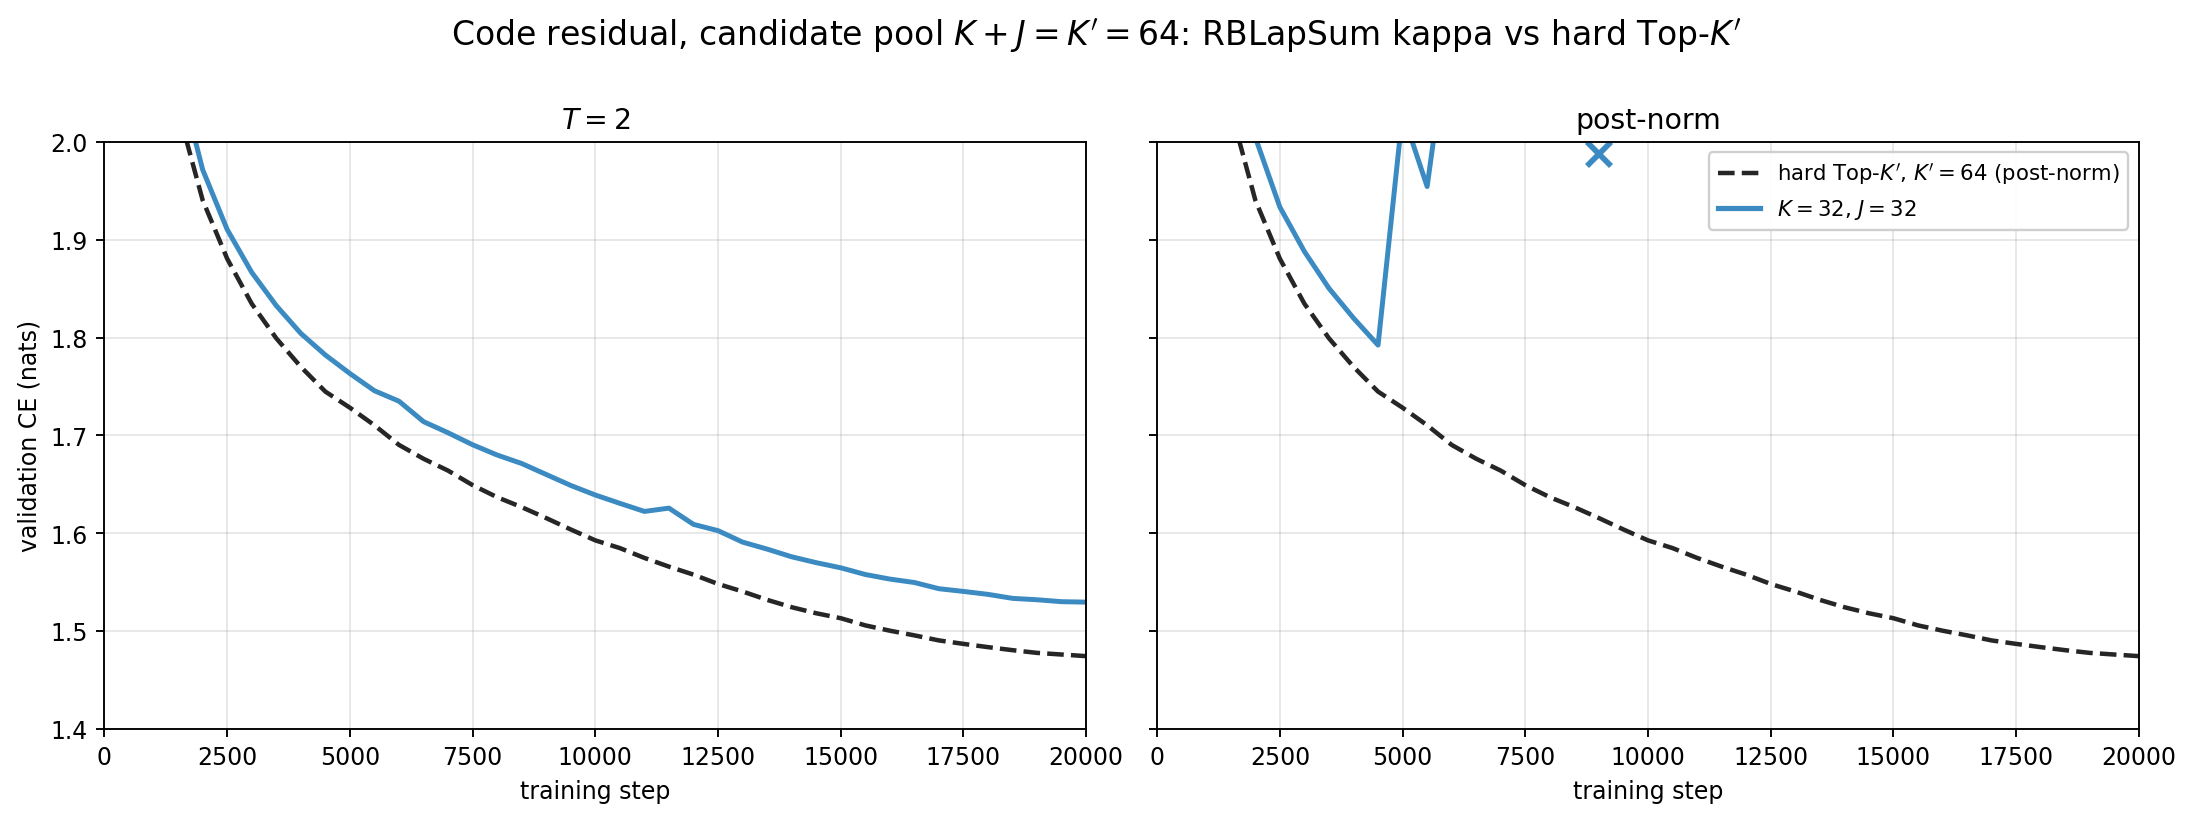
\includegraphics[width=\textwidth]{figures/kj-cr/cr_pool_k64.png}
\caption{$\Kp = 64$, code carried. The single surrogate cell $(32,32)$ ends
$0.055$ above hard Top-64 at $T=2$ (in the stream grid it ended $0.010$
below); the post-norm cell is the one that collapsed from step 4900 and was
stopped at 9160 (the cross marks the stop).}
\end{figure}

\begin{figure}[htb]\centering
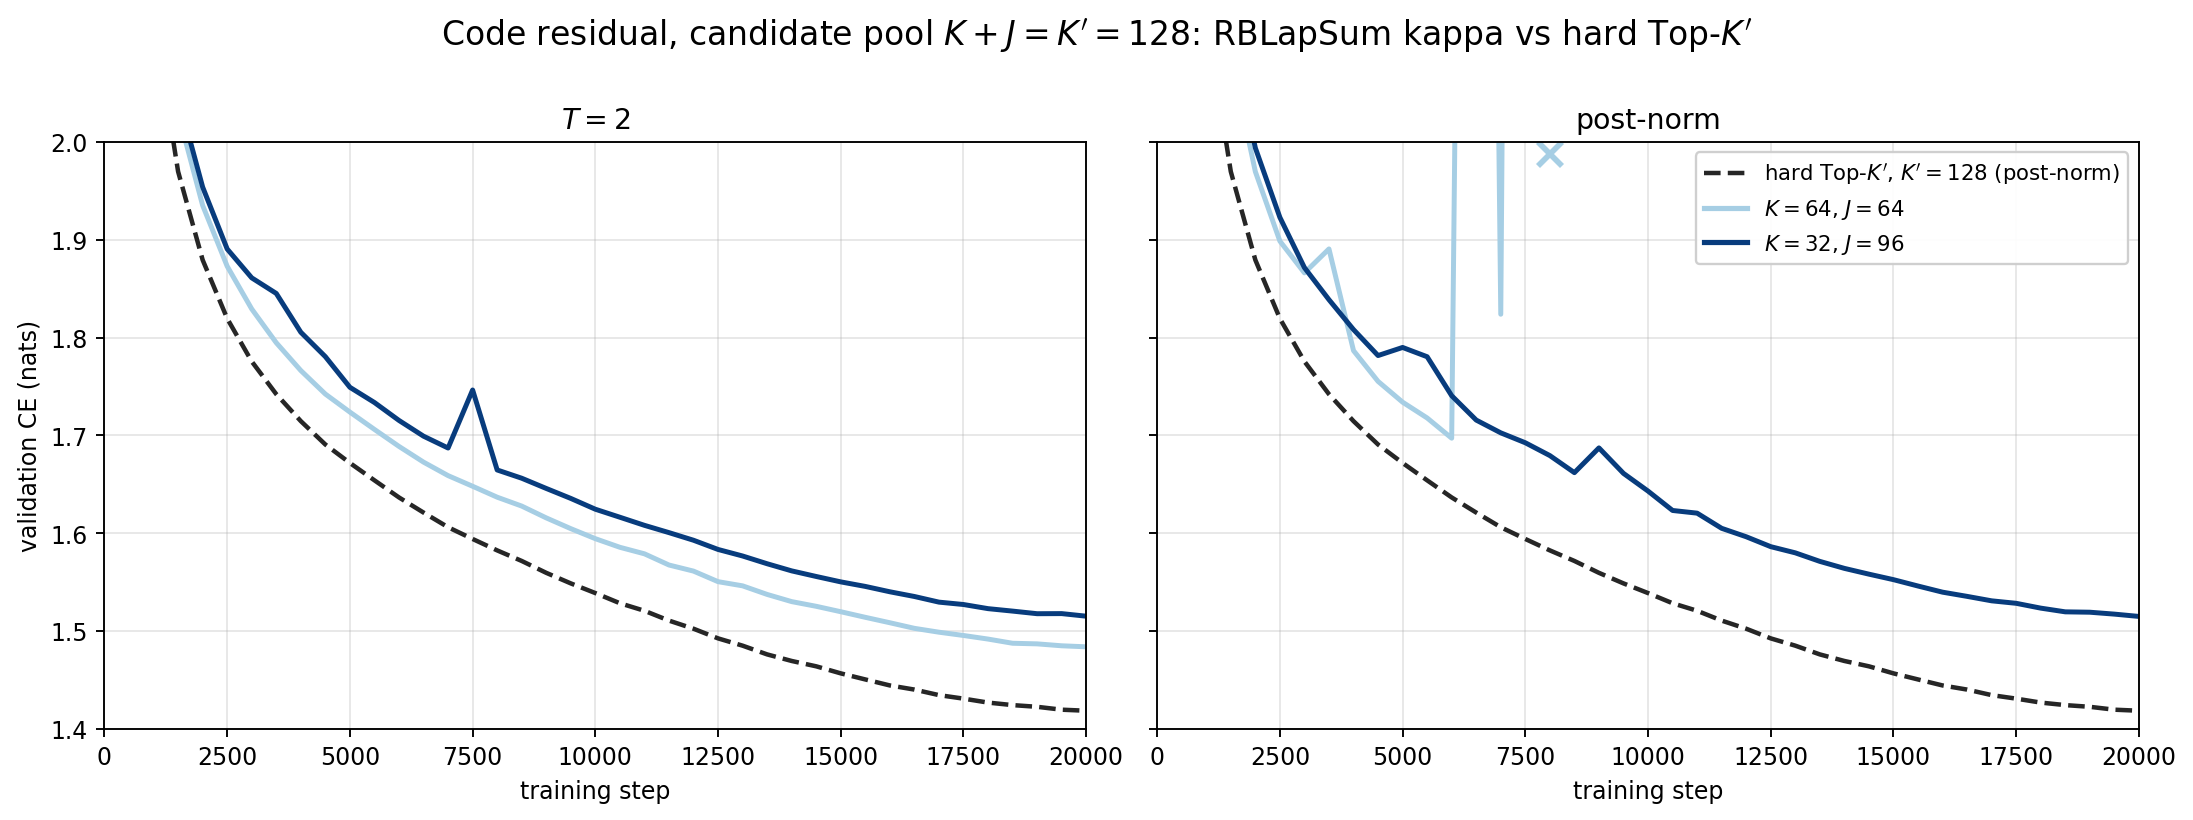
\includegraphics[width=\textwidth]{figures/kj-cr/cr_pool_k128.png}
\caption{$\Kp = 128$, code carried. At $T=2$ both cells sit above hard
Top-128 throughout, $(64,64)$ by $0.065$ and $(32,96)$ by $0.097$ at the
end, with the ordering by $K$ of the stream grid; the $(32,96)$ curve shows a
recovered spike at step 7500. Under the post-norm $(64,64)$ collapsed at
step 8020 and $(32,96)$ finished at $1.5151$ with recovered spikes at steps
4500, 9000 and 11000.}
\end{figure}

\begin{figure}[htb]\centering
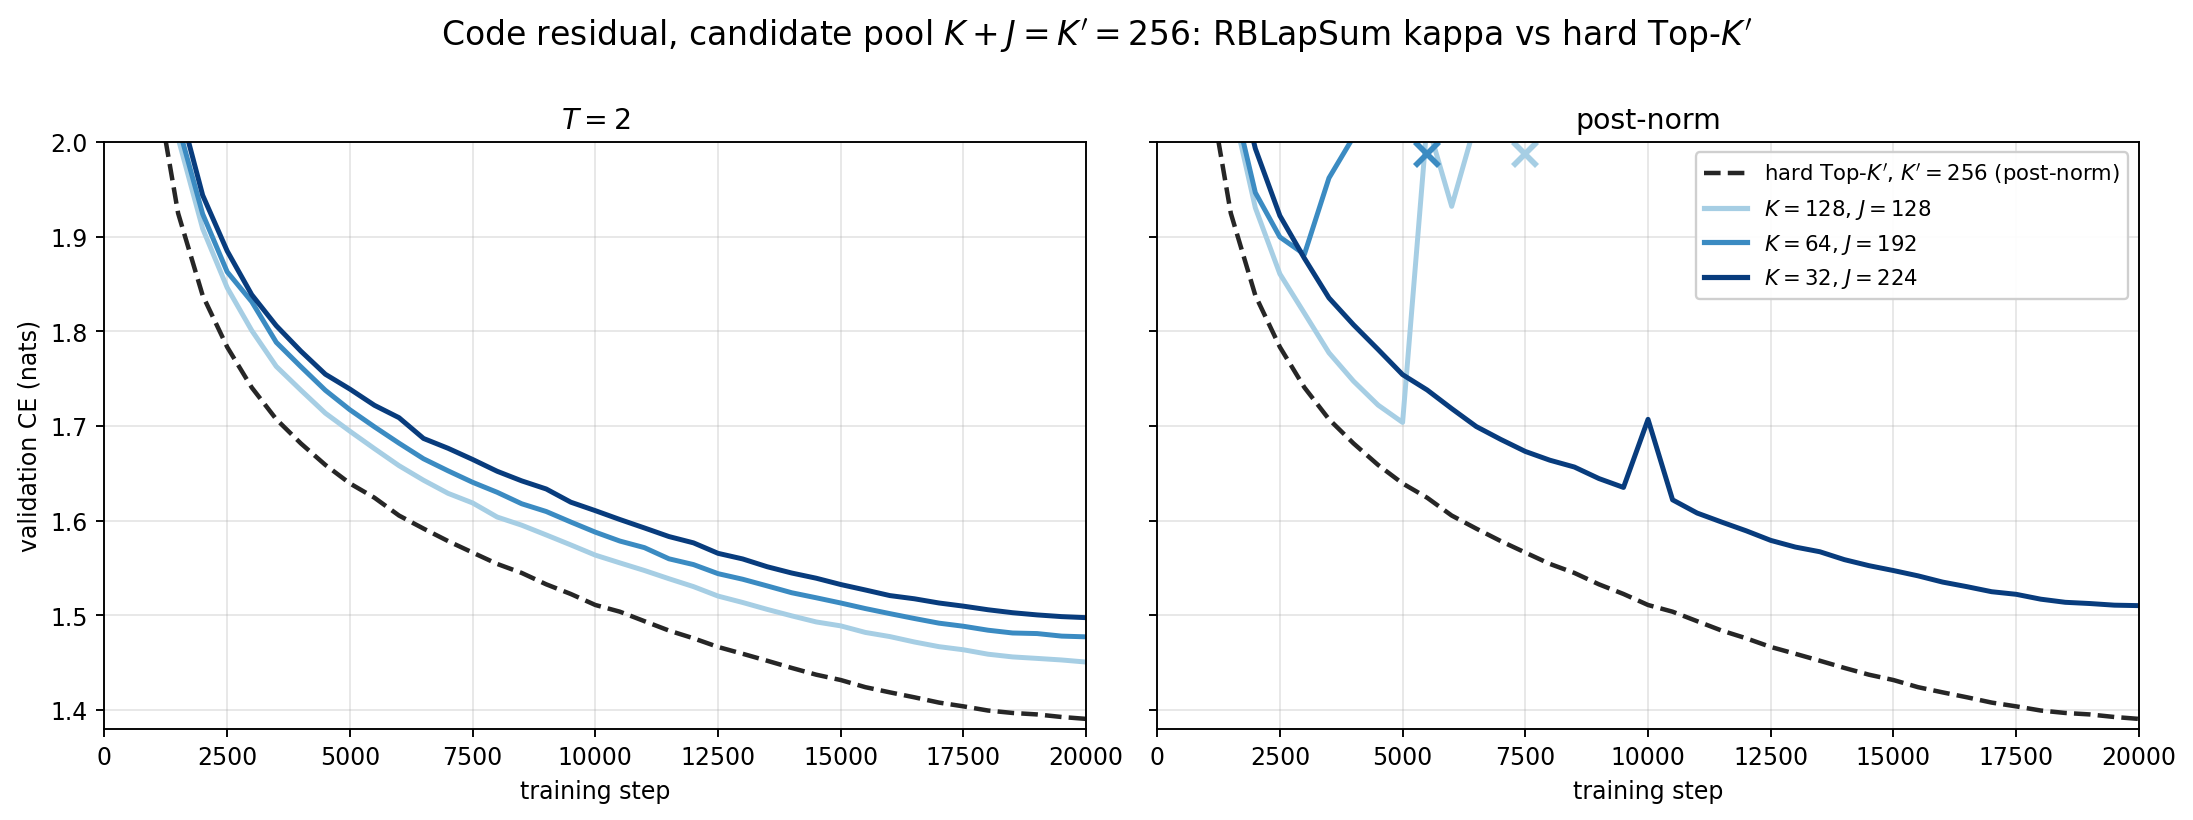
\includegraphics[width=\textwidth]{figures/kj-cr/cr_pool_k256.png}
\caption{$\Kp = 256$, code carried. At $T=2$ the three cells order by $K$
-- $1.4507$, $1.4773$, $1.4976$ for $K = 128, 64, 32$ -- and all lie above
hard Top-256 ($1.3907$) from the first validation point on. Under the
post-norm $(128,128)$ and $(64,192)$ collapsed (stopped at 7960 and 5840)
and $(32,224)$ finished at $1.5103$ after a spike at step 10000.}
\end{figure}

\begin{figure}[htb]\centering
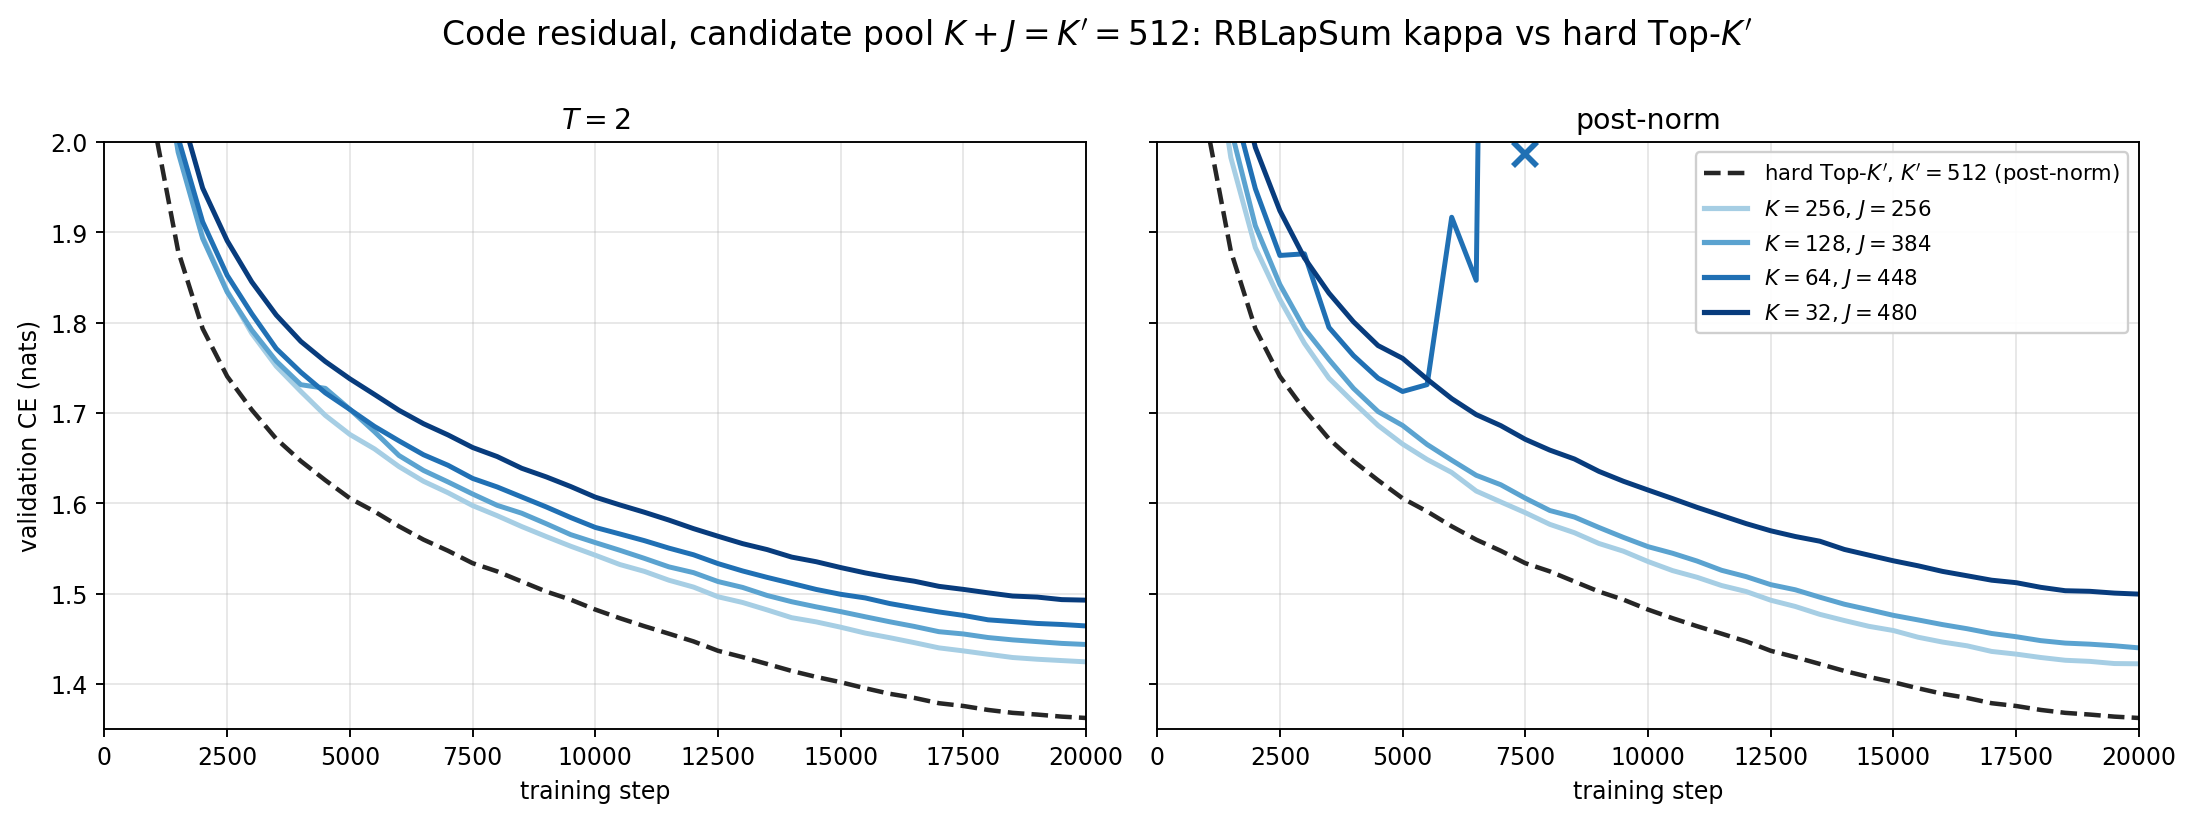
\includegraphics[width=\textwidth]{figures/kj-cr/cr_pool_k512.png}
\caption{$\Kp = 512$, code carried. The ordering is monotone in $K$ in both
variants and every cell lies above hard Top-512 ($1.3622$): at $T=2$ by
$0.062$ ($K=256$), $0.081$ ($128$), $0.102$ ($64$) and $0.131$ ($32$). Under
the post-norm $(64,448)$ collapsed at step 7860; the other three finished,
and $(32,480)$ is no longer a reversal.}
\end{figure}

\subsection*{Per active count}

Each figure fixes $K$ and shows every candidate window trained at that $K$
(solid, blue ramp light to dark with increasing $J$) against all five hard
Top-$\Kp$ baselines (dashed, red ramp light to dark with increasing $\Kp$).
All runs are code-carried.

\begin{figure}[htb]\centering
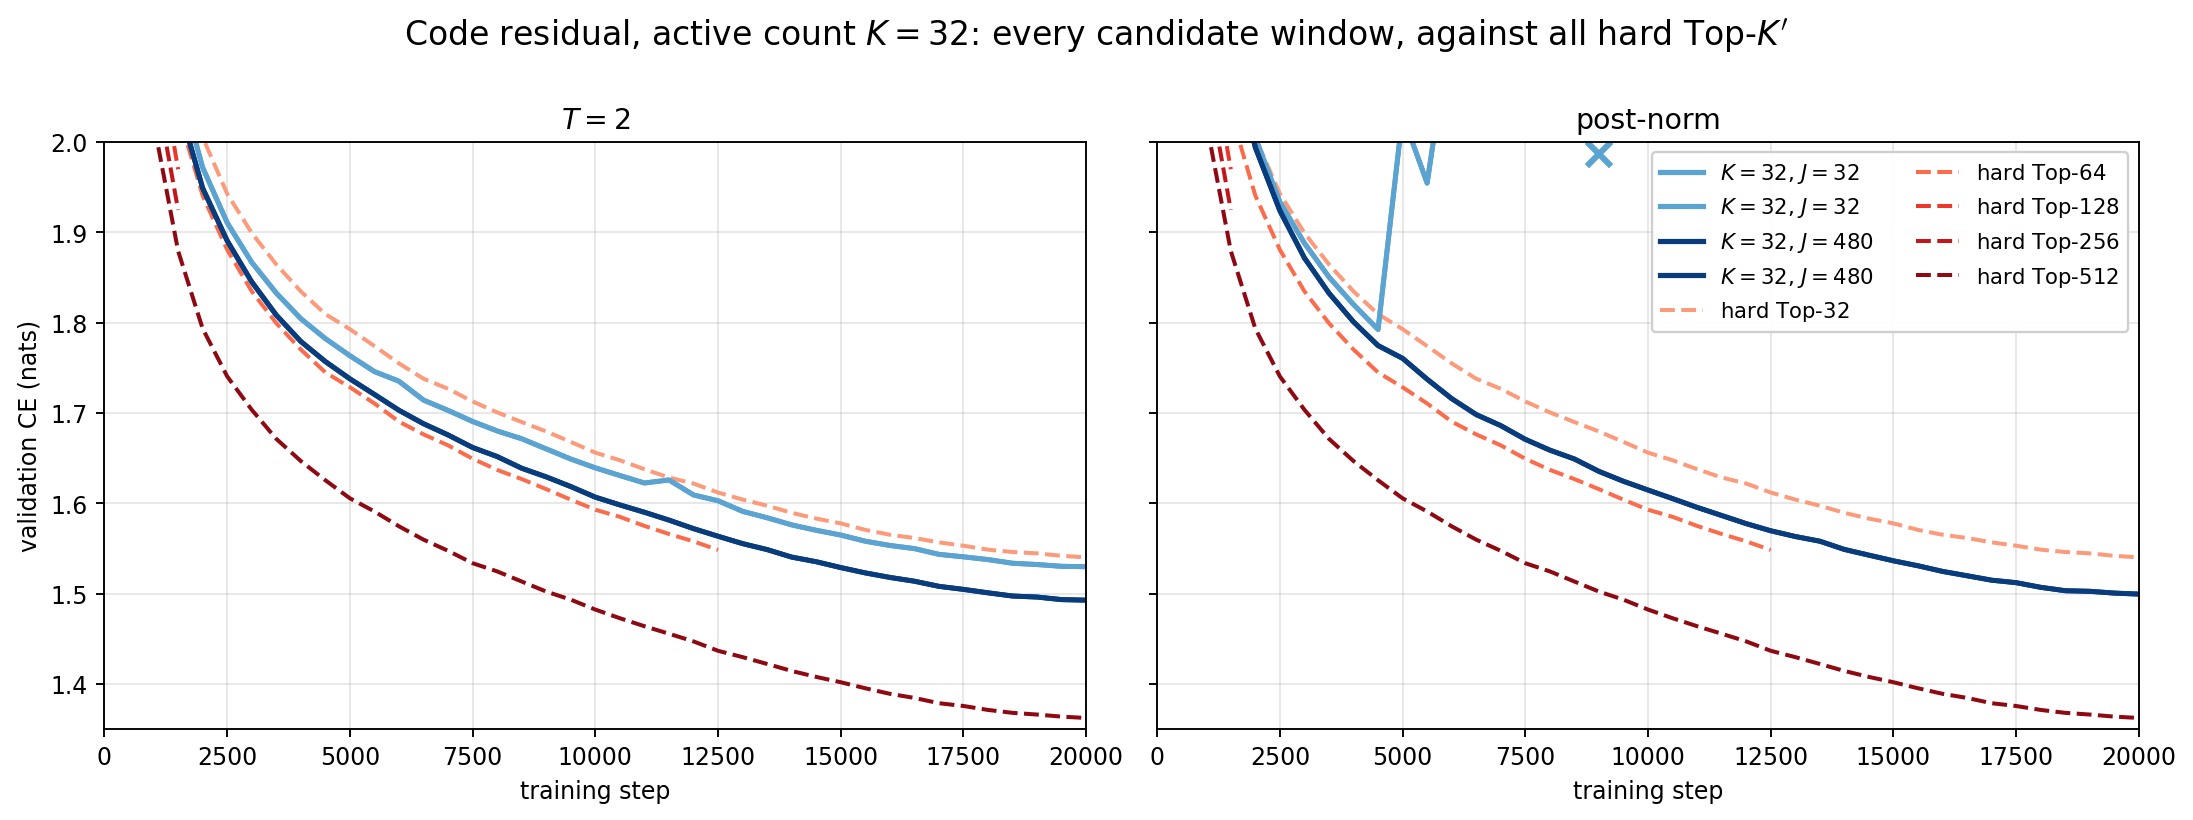
\includegraphics[width=\textwidth]{figures/kj-cr/cr_active_k32.png}
\caption{$K = 32$, code carried. Widening the window lowers the loss
monotonically in both variants, but the hard ladder has moved down with the
carry: the widest window ends between hard Top-32 ($1.5400$) and hard Top-64
($1.4745$), where the stream-carried $J=224$ cell had passed hard Top-128.
The post-norm $(32,32)$ cell collapsed; the other three post-norm cells track
the $T=2$ ones to within $0.013$.}
\end{figure}

\begin{figure}[htb]\centering
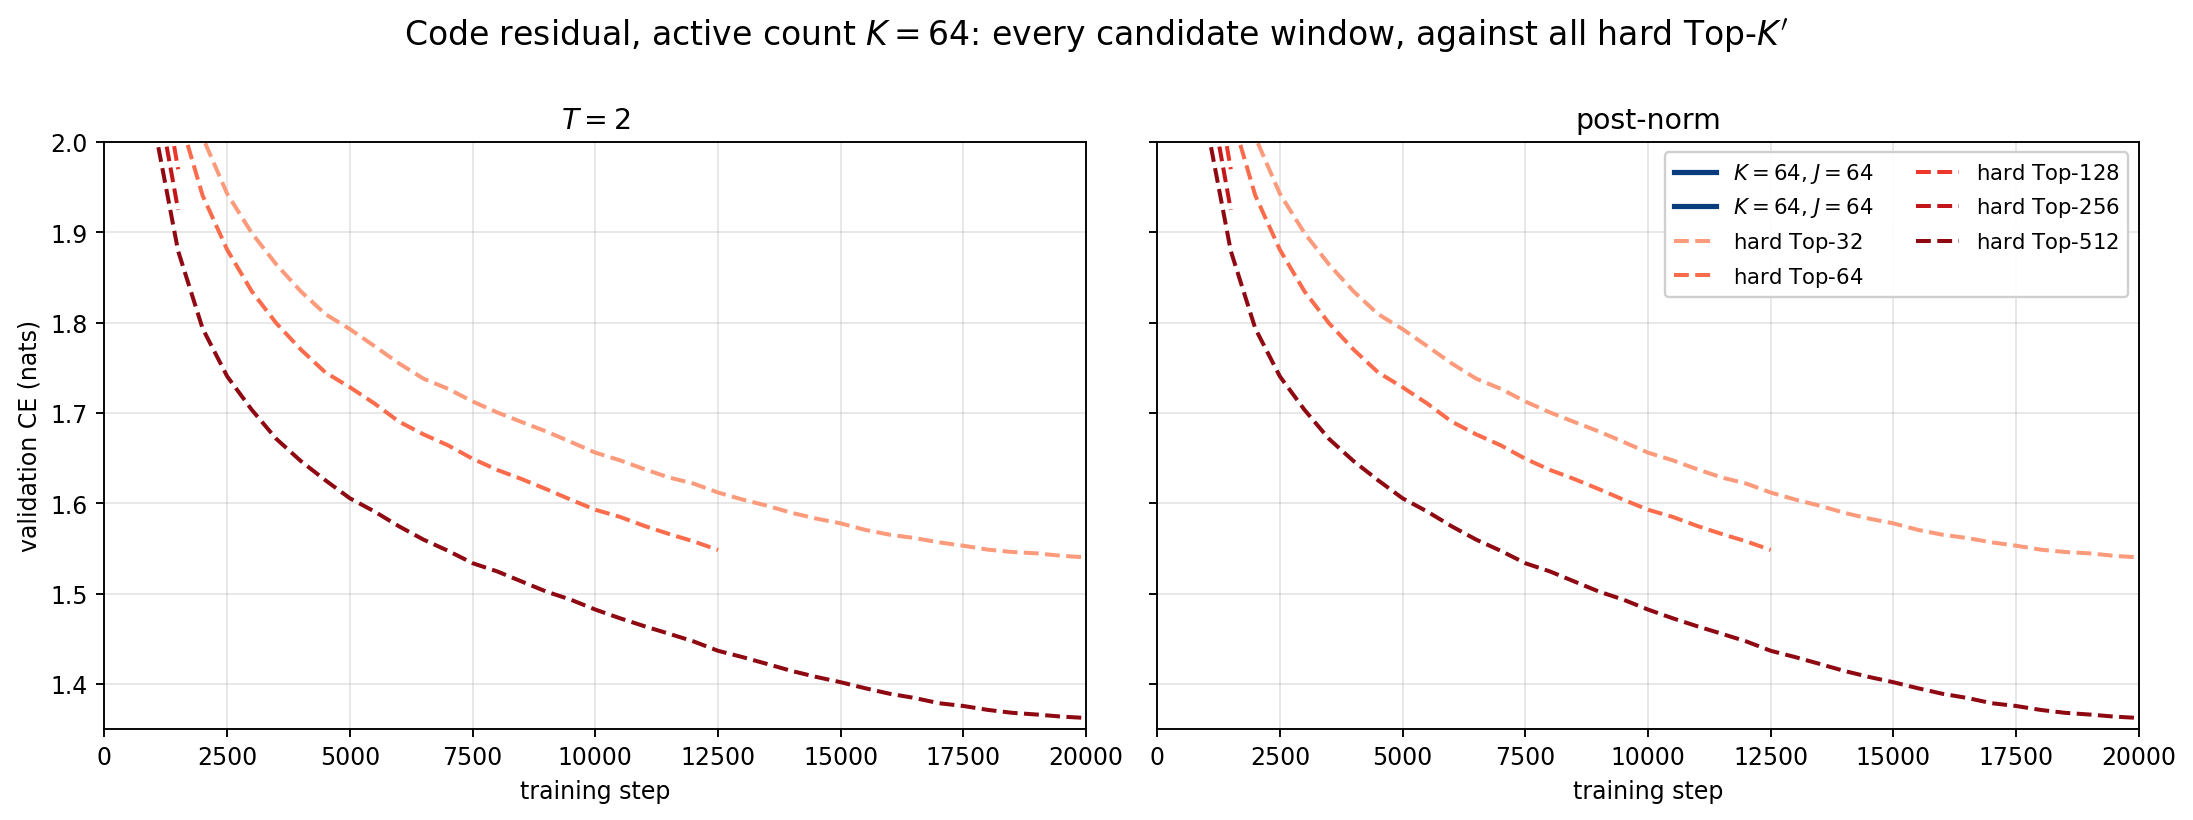
\includegraphics[width=\textwidth]{figures/kj-cr/cr_active_k64.png}
\caption{$K = 64$, code carried. At $T=2$ only the widest window,
$J=448$, ends below hard Top-64, by $0.010$; $J = 64$ and $192$ end above it.
All three post-norm cells collapsed between steps 5840 and 8020.}
\end{figure}

\begin{figure}[htb]\centering
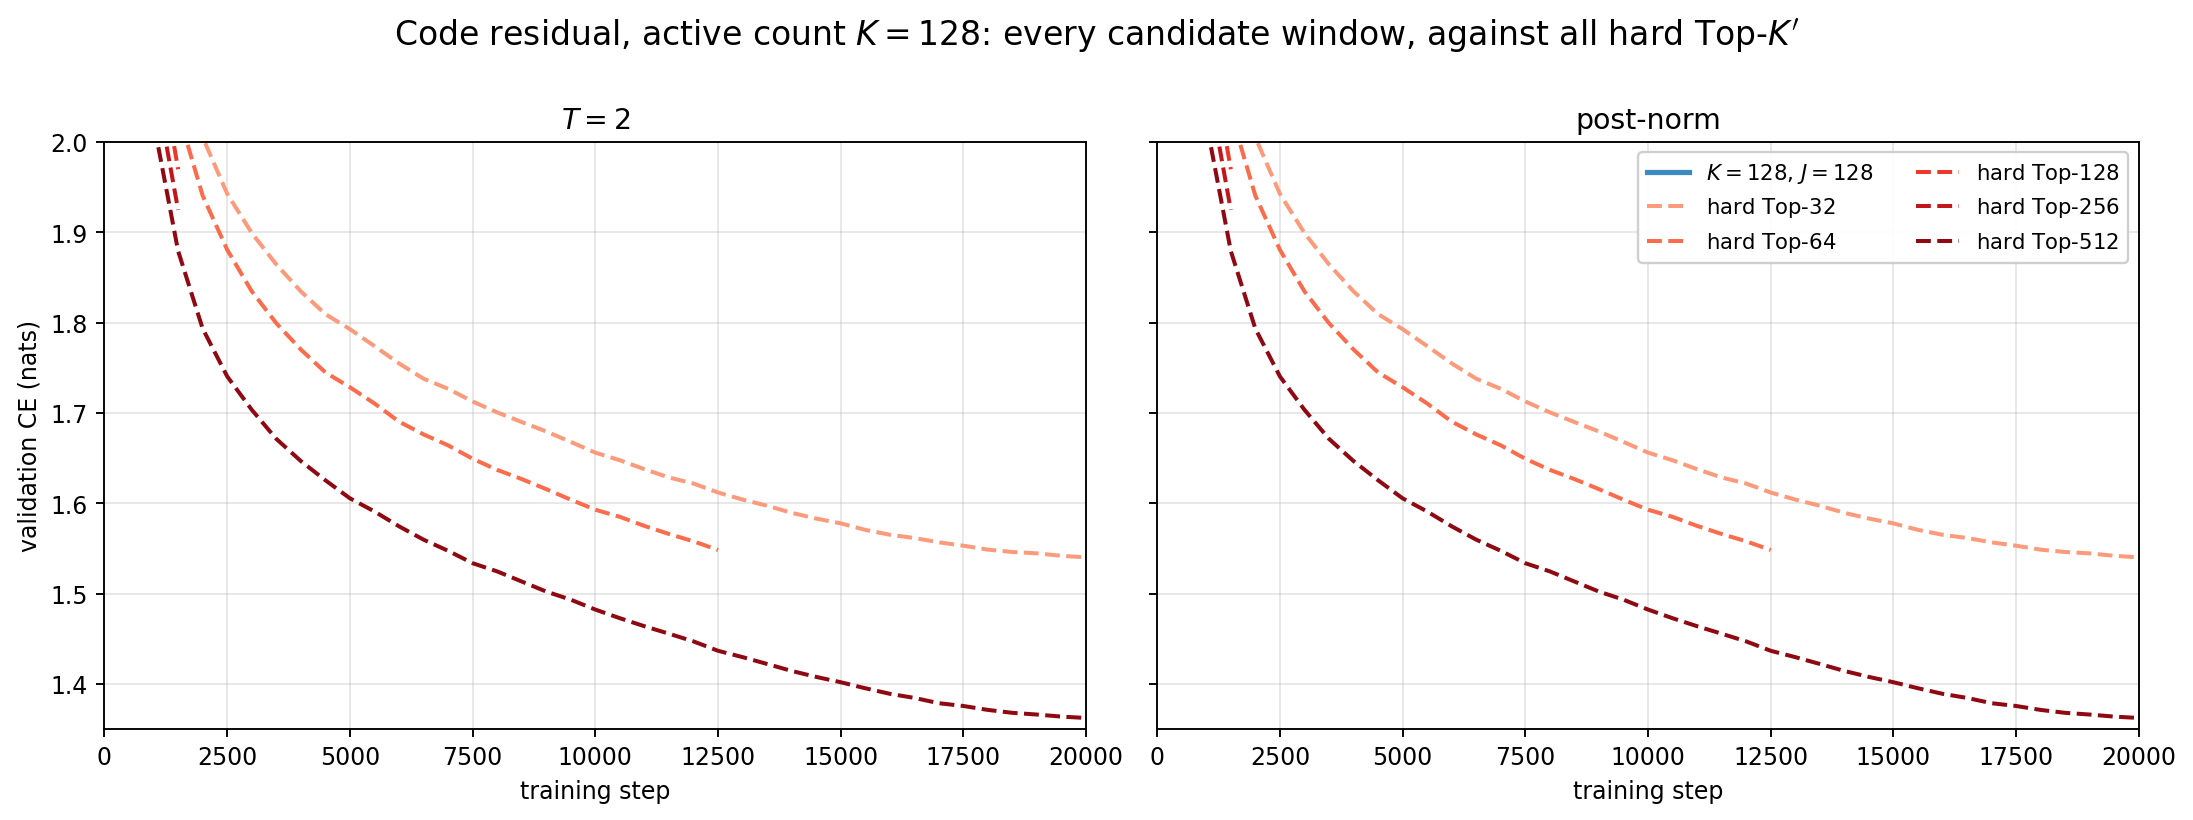
\includegraphics[width=\textwidth]{figures/kj-cr/cr_active_k128.png}
\caption{$K = 128$, code carried. Both $T=2$ cells and the surviving
post-norm cell end above hard Top-128 ($1.4187$), by $0.032$ ($J=128$),
$0.025$ and $0.021$ ($J=384$, $T=2$ and post-norm); in the stream grid both
windows beat hard Top-256. The post-norm $(128,128)$ cell collapsed at step
7960.}
\end{figure}

\begin{figure}[htb]\centering
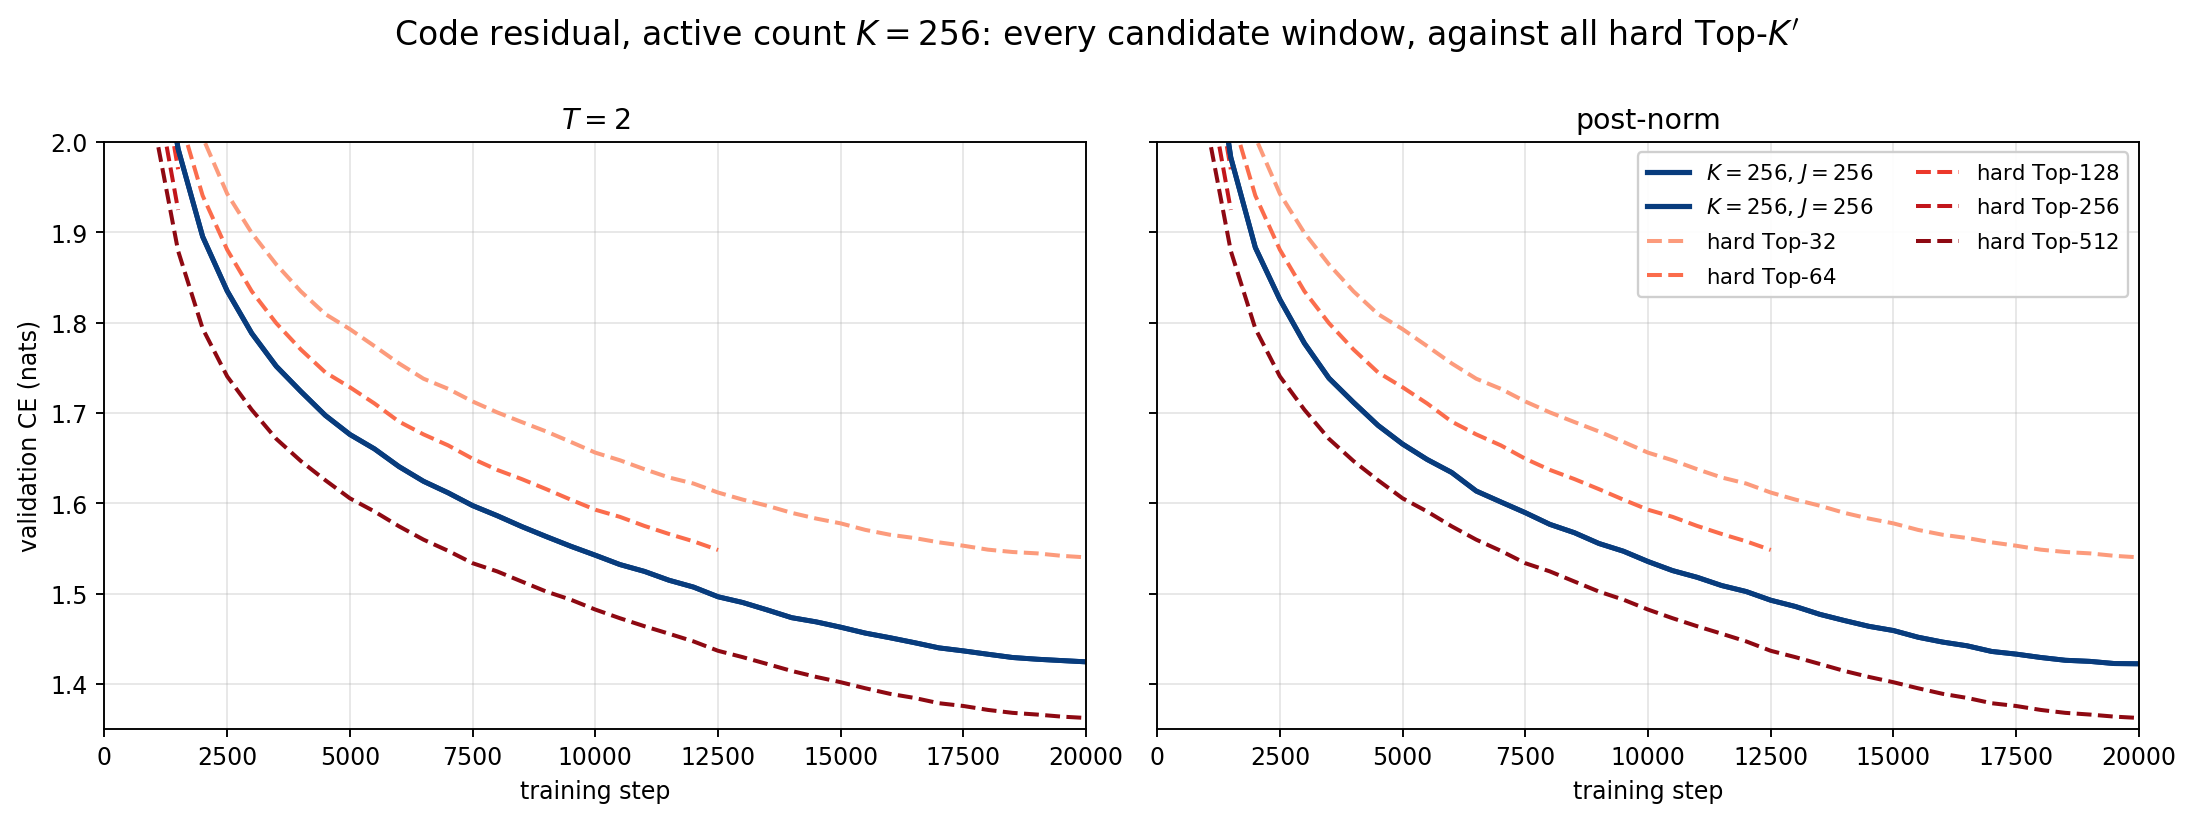
\includegraphics[width=\textwidth]{figures/kj-cr/cr_active_k256.png}
\caption{$K = 256$, code carried. The single cell ends at $1.4244$
($T=2$) and $1.4222$ (post-norm), above hard Top-256 ($1.3907$) by $0.034$
and $0.032$ and above hard Top-512 by $0.06$. The stream-carried version of
this cell, $1.4146$, was the best model of the K+J note; code-carried hard
Top-256 and Top-512 are both below it.}
\end{figure}

% ============================================================
\section{Stream carried versus code carried}
% ============================================================

The same cell in the two families, the difference being the carry from
block 1 on. Final validation CE, code carried minus stream carried
(negative: the code residual is better):

\begin{center}\small
\begin{tabular}{lcccc}
\toprule
$T=2$: $K$ & $\Kp{=}64$ & $\Kp{=}128$ & $\Kp{=}256$ & $\Kp{=}512$ \\
\midrule
$32$   & $-0.0196$ & $+0.0007$ & $+0.0134$ & $-0.0016$ \\
$64$   & ---       & $-0.0301$ & $-0.0148$ & $-0.0086$ \\
$128$  & ---       & ---       & $-0.0295$ & $-0.0162$ \\
$256$  & ---       & ---       & ---       & $-0.0181$ \\
\midrule
post-norm: $K$ & & & & \\
\midrule
$32$   & div       & $+0.0035$ & $+0.0154$ & $-0.0376$ \\
$64$   & ---       & div       & div       & div \\
$128$  & ---       & ---       & div       & $+0.0104$ \\
$256$  & ---       & ---       & ---       & $+0.0076$ \\
\midrule
hard Top-$\Kp$ & $-0.0664$ & $-0.0751$ & $-0.0653$ & $-0.0609$ \\
\bottomrule
\end{tabular}
\end{center}

Hard Top-32 moves by $-0.0621$. The two families differ by one operation
from block 1 on, and that operation is worth $0.06$--$0.075$ nats to a hard
bottleneck and $-0.030$ to $+0.015$ to the surrogate ($T=2$ mean $-0.012$;
the surviving post-norm cells $-0.038$ to $+0.015$). The surrogate's
diagonal cells gain the most ($-0.020$ to $-0.030$ at $J = K \le 128$),
the wide windows of $K=32$ nothing.

\subsection*{Hard Top-$\Kp$}

Carrying the code lowers the final loss of every hard baseline by nearly the
same amount, $0.061$ to $0.075$ nats: $1.6022 \to 1.5400$ at $\Kp = 32$,
$1.5408 \to 1.4745$ at $64$, $1.4938 \to 1.4187$ at $128$, $1.4560 \to 1.3907$
at $256$ and $1.4232 \to 1.3622$ at $512$. The gain is largest early and
narrows: at step 2500 the code-carried Top-32 and Top-512 lead their
stream-carried twins by $0.107$ and $0.102$, at step 20000 by $0.062$ and
$0.061$. Measured against the stream-carried ladder, a code-carried Top-$\Kp$
lands at or below the stream-carried Top-$2\Kp$: $1.5400$ against $1.5408$
($\Kp = 32$ vs.\ $64$), $1.4745$ against $1.4938$ ($64$ vs.\ $128$), $1.4187$
against $1.4560$ ($128$ vs.\ $256$) and $1.3907$ against $1.4232$ ($256$ vs.\
$512$); the code-carried Top-128 ($1.4187$) also matches the stream-carried
Top-512 ($1.4232$). The carry is thus worth at least one doubling of the
active count for a hard bottleneck, at every scale tested.

\begin{figure}[htb]\centering
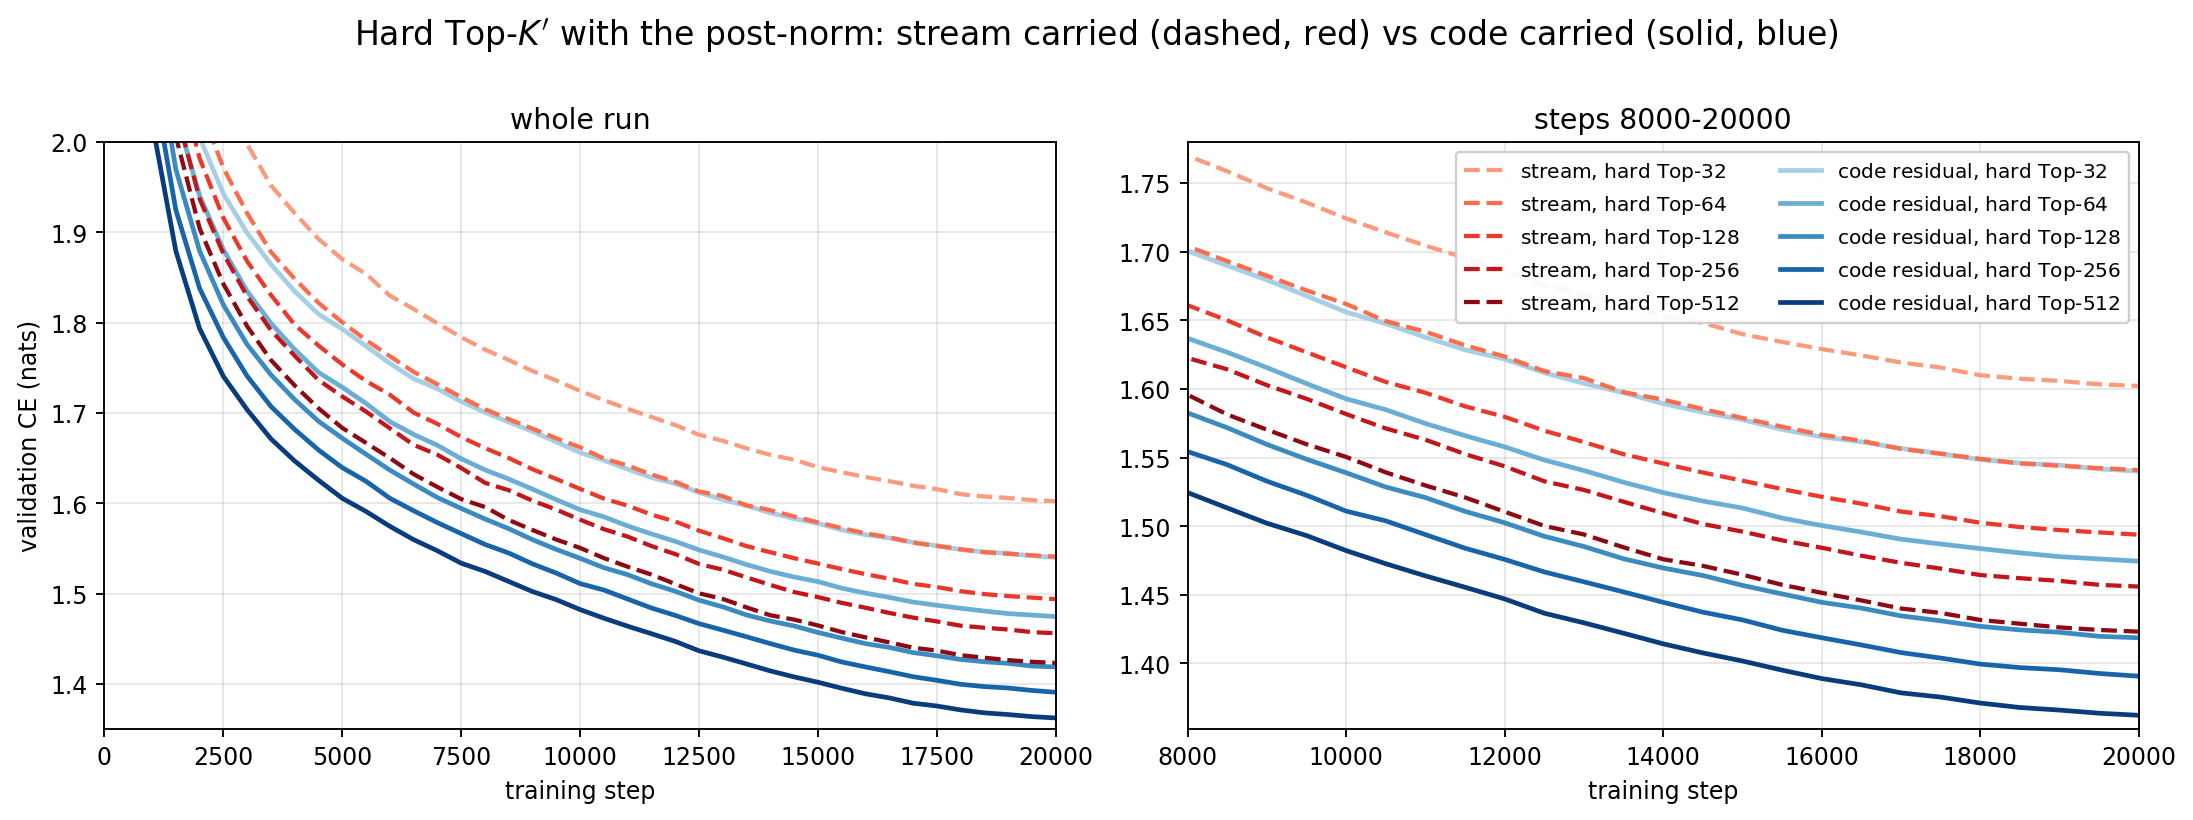
\includegraphics[width=\textwidth]{figures/kj-cr/cr_vs_stream_hard.png}
\caption{Hard Top-$\Kp$ with the post-norm, $\Kp = 32$ to $512$: stream
carried (dashed, red ramp light to dark with $\Kp$) and code carried (solid,
blue ramp). Left the whole run, right the last 12k steps on a tight scale.
Every solid curve lies below the dashed curve of the same shade from the first
validation point on, and the solid curve of each $\Kp$ runs along the dashed
curve of $2\Kp$: code-carried Top-32 and stream-carried Top-64 are
indistinguishable after step 12000.}
\end{figure}

\subsection*{RBLapSum, per active count}

Each figure fixes $K$ and shows every $J$ trained at that $K$ in both
families: stream carried (dashed, red ramp light to dark with $J$) and code
carried (solid, blue ramp); left panel $T=2$, right panel post-norm.

\begin{figure}[htb]\centering
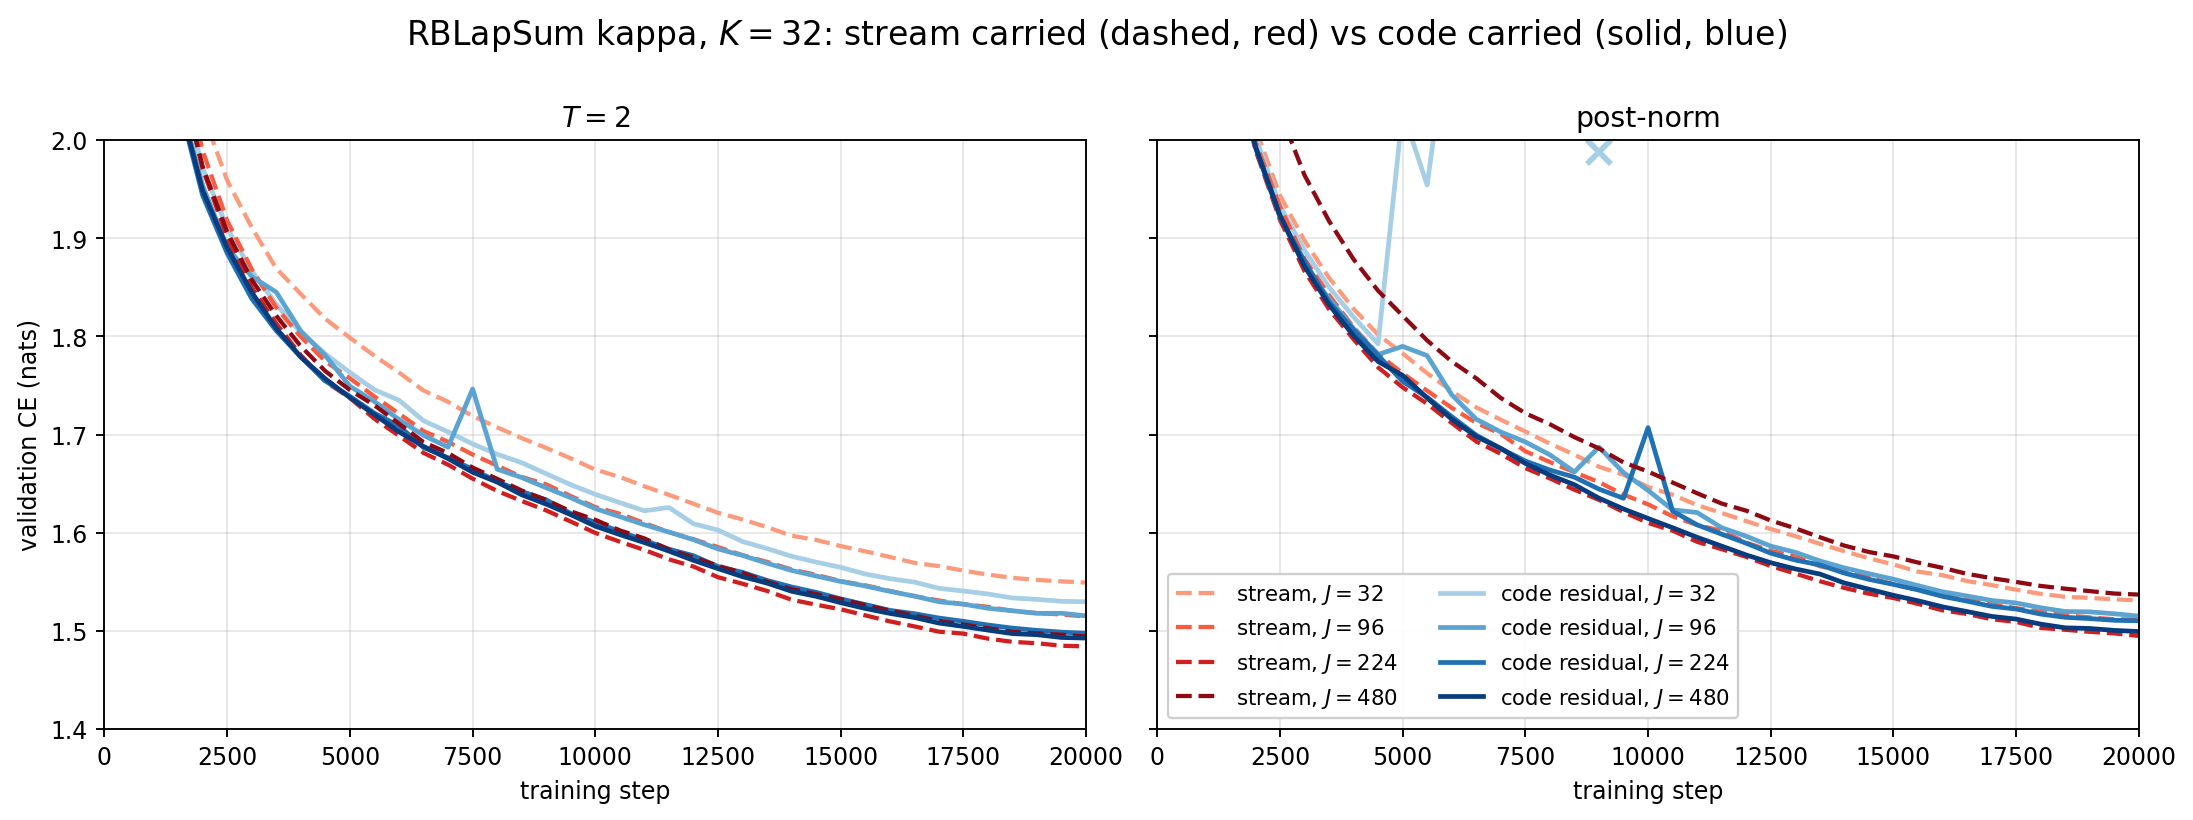
\includegraphics[width=\textwidth]{figures/kj-cr/cr_vs_stream_rbk_k32.png}
\caption{$K = 32$, $J \in \{32, 96, 224, 480\}$. At $T=2$ each
code-carried curve runs within $0.02$ of its stream-carried twin, below it
for $J=32$ and above for $J=224$; the carried $J=32$ cell shows recovered
spikes at steps 4500 and 11500. Under the post-norm the carried $(32,32)$
cell collapsed, $J = 96$ and $224$ end within $0.016$ of their twins, and
$J=480$ ends $0.038$ below its twin, the stream grid's reversal.}
\end{figure}

\begin{figure}[htb]\centering
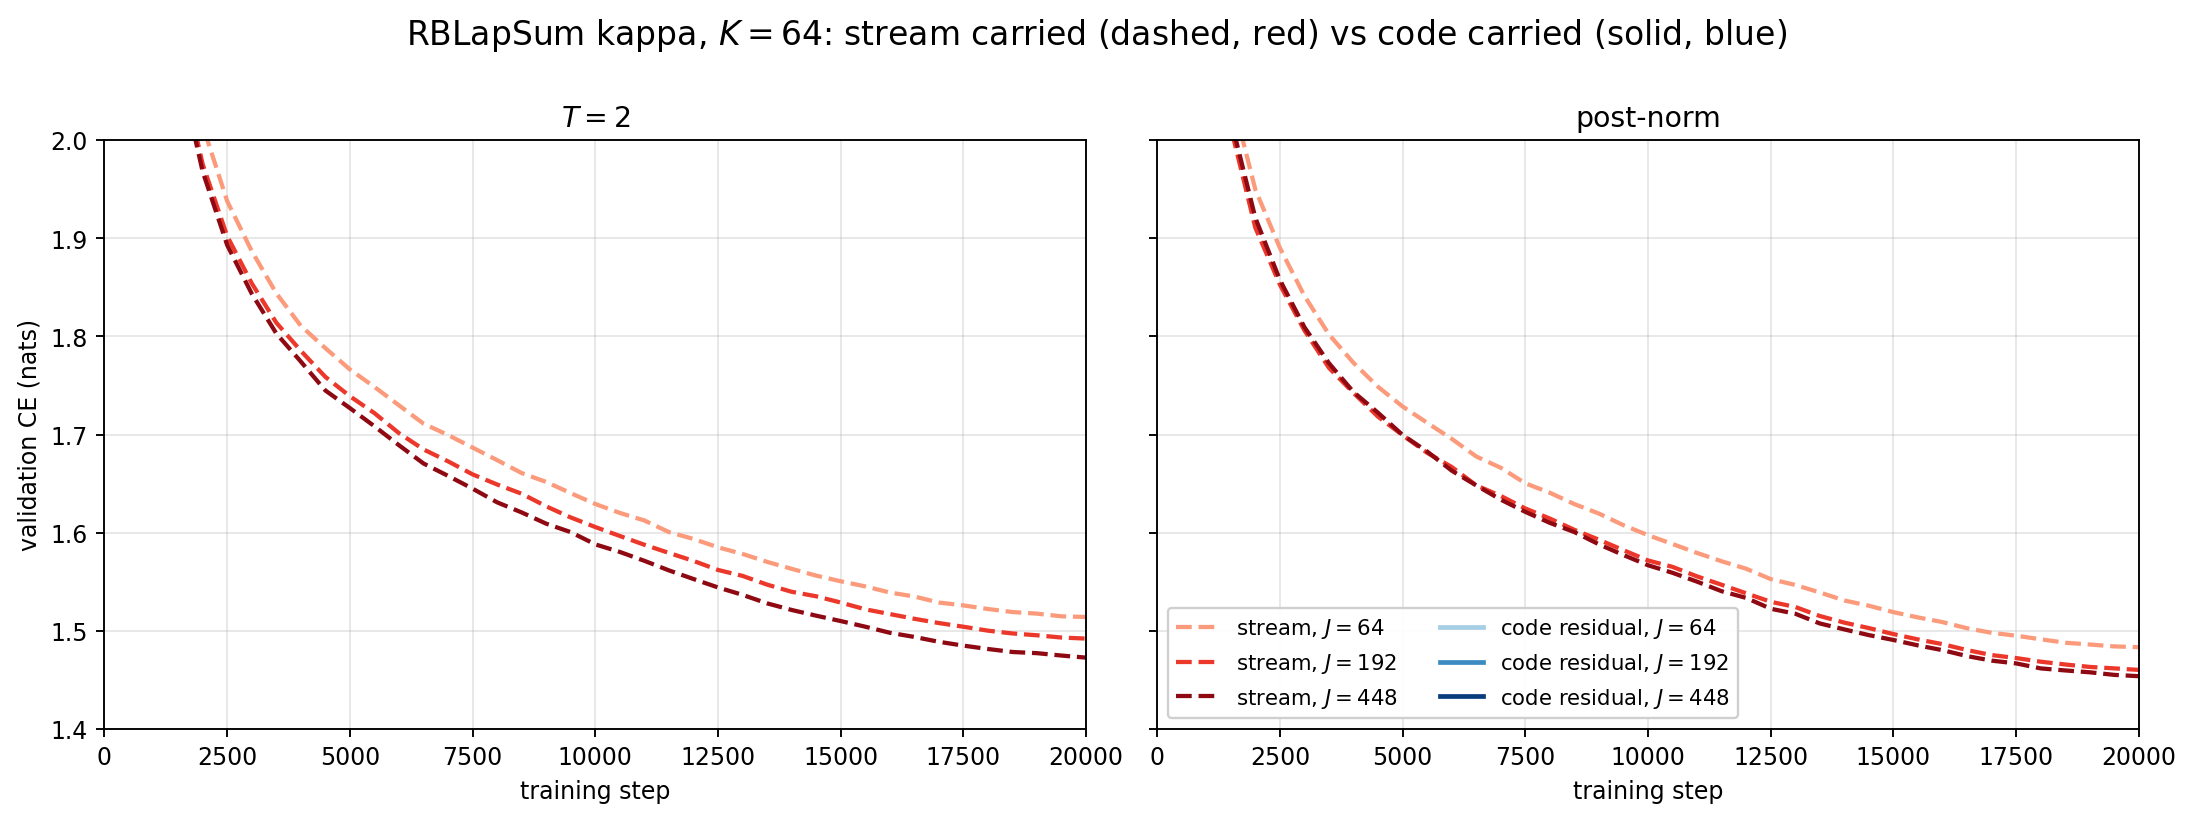
\includegraphics[width=\textwidth]{figures/kj-cr/cr_vs_stream_rbk_k64.png}
\caption{$K = 64$, $J \in \{64, 192, 448\}$. At $T=2$ all three
code-carried cells lie below their twins from about step 2500 on and end
$0.030$, $0.015$ and $0.009$ lower; the gap narrows as training proceeds.
Under the post-norm all three code-carried cells collapsed (stopped at 8020,
5840 and 7860) while the stream-carried ones trained smoothly.}
\end{figure}

\begin{figure}[htb]\centering
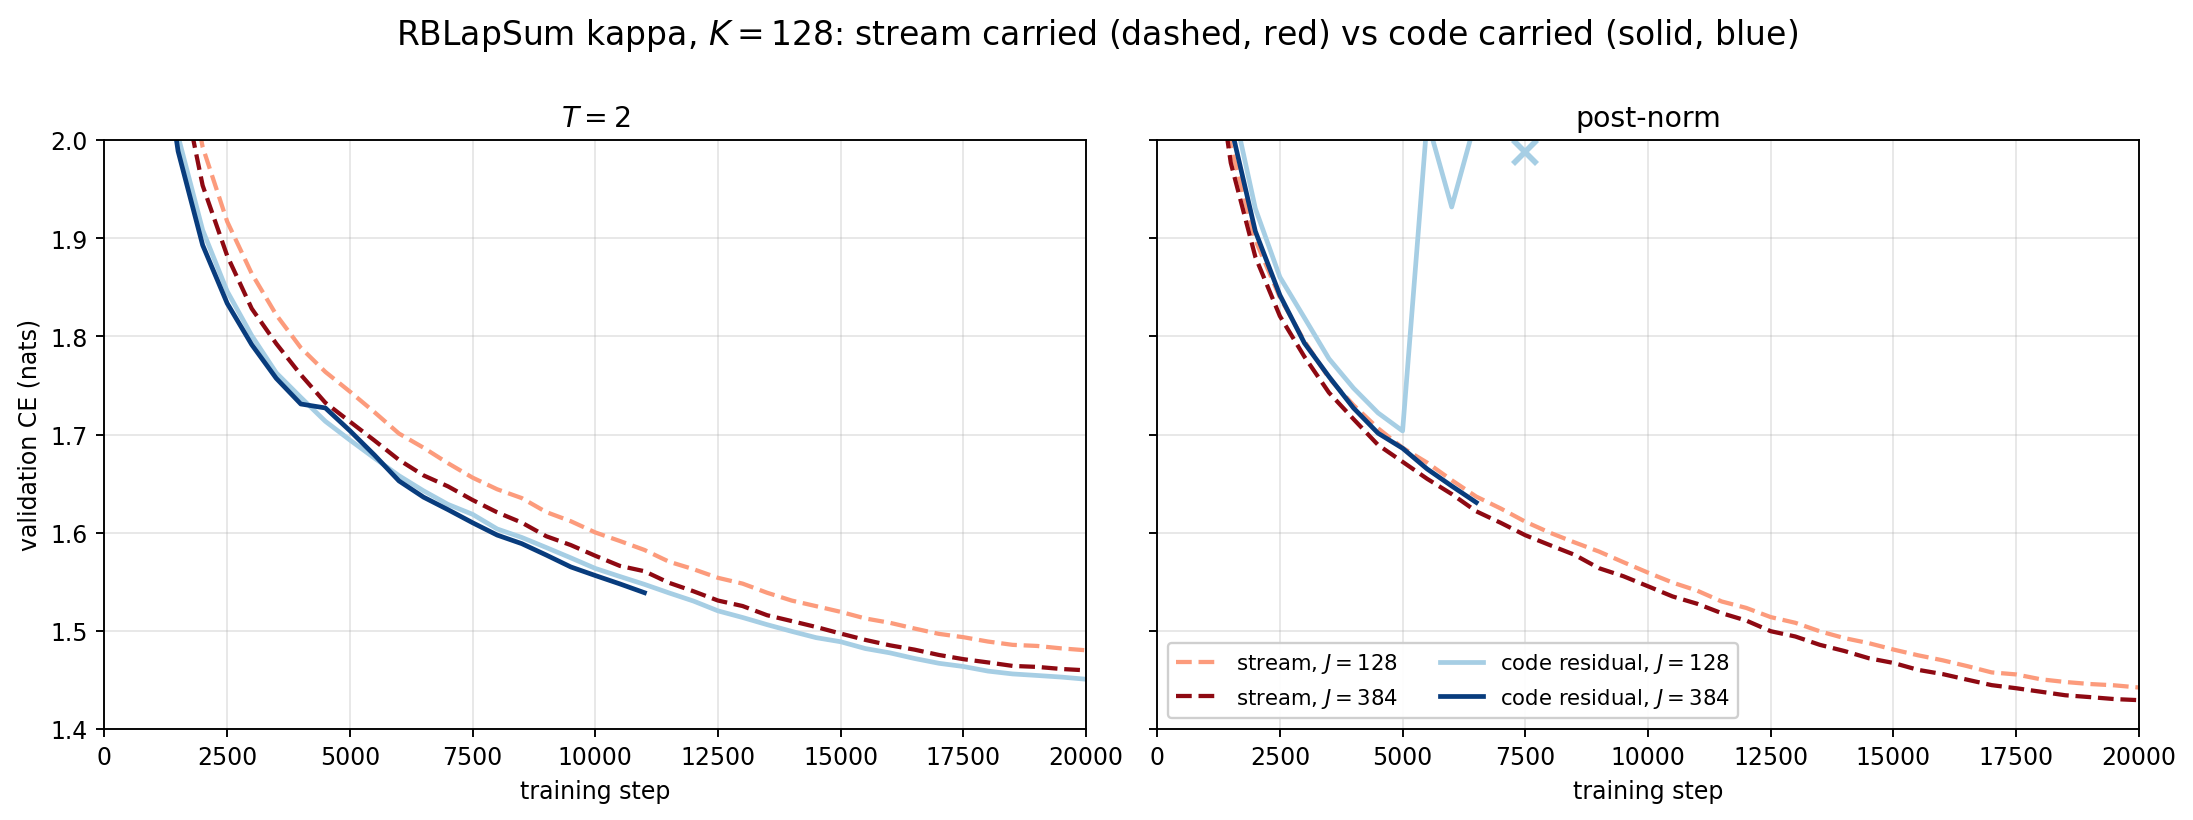
\includegraphics[width=\textwidth]{figures/kj-cr/cr_vs_stream_rbk_k128.png}
\caption{$K = 128$, $J \in \{128, 384\}$. At $T=2$ the code-carried
cells end $0.030$ and $0.016$ below their twins, separating from about step
5000. Under the post-norm $(128,128)$ collapsed at step 7960 and the
$(128,384)$ curves are indistinguishable ($+0.010$ at the end).}
\end{figure}

\begin{figure}[htb]\centering
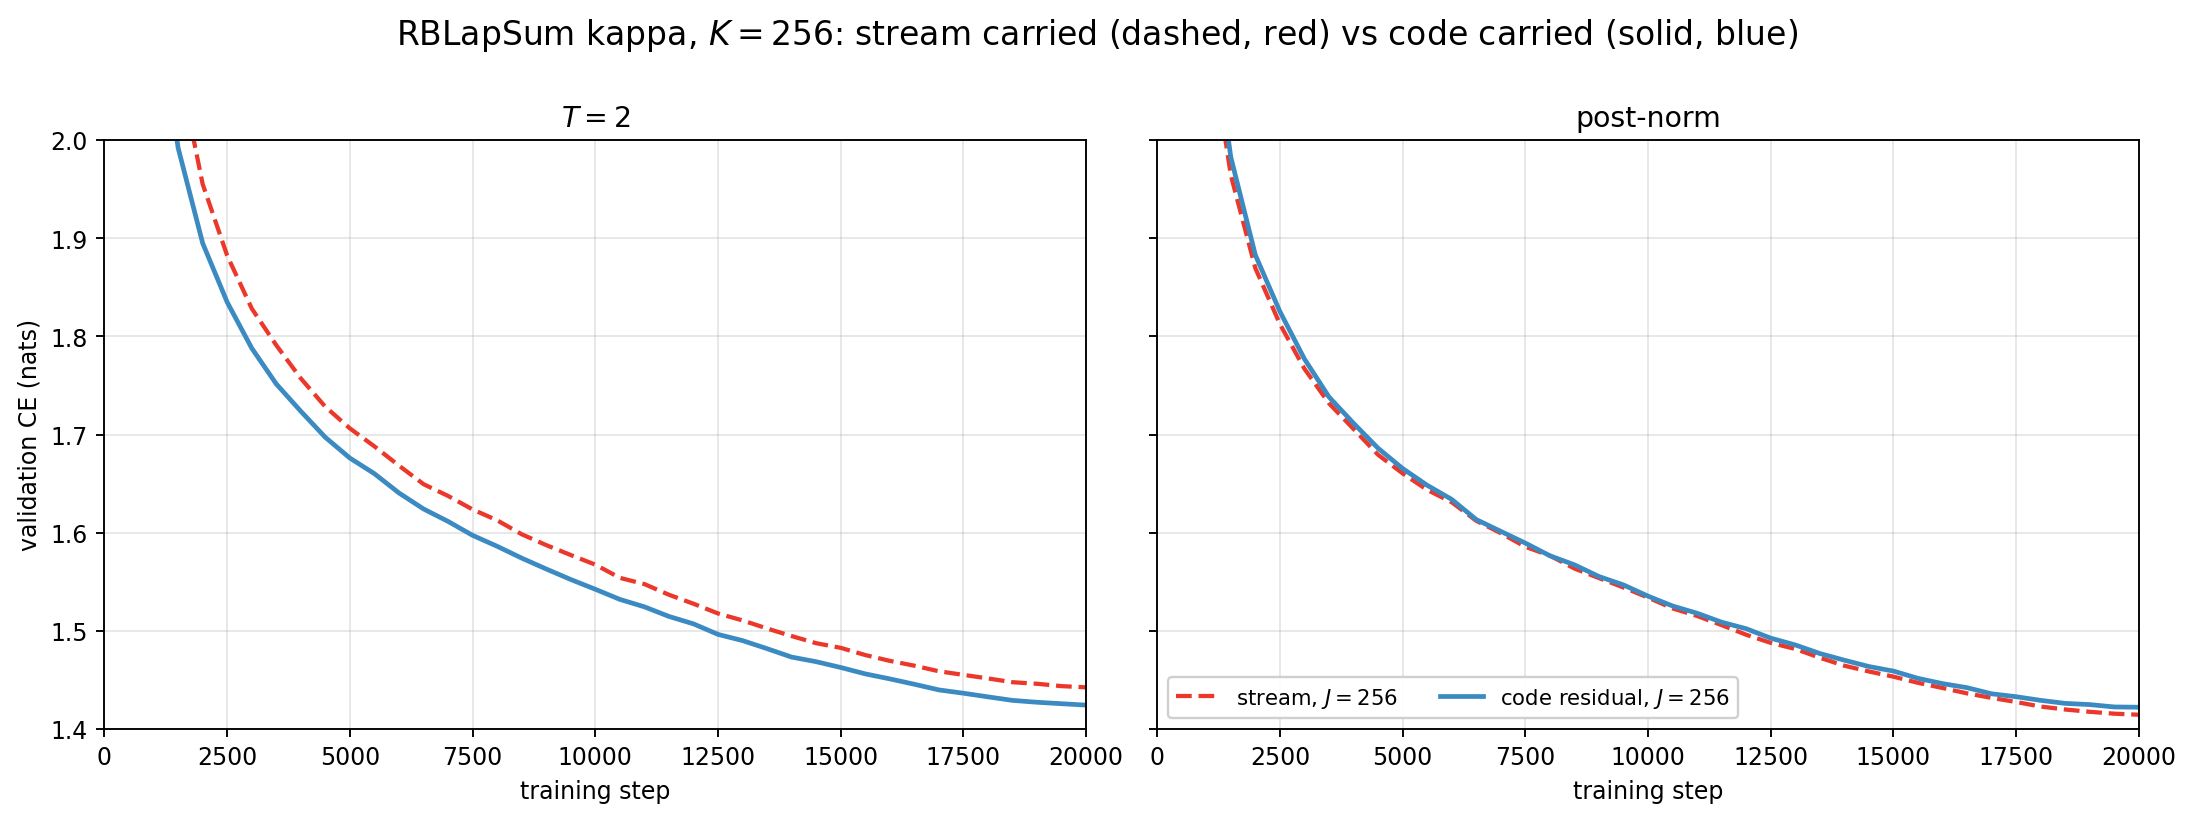
\includegraphics[width=\textwidth]{figures/kj-cr/cr_vs_stream_rbk_k256.png}
\caption{$K = 256$, $J = 256$. $T=2$: the code-carried cell leads
throughout and ends $0.018$ lower; post-norm: the two curves coincide to
within $0.008$ at every point.}
\end{figure}

% ============================================================
\section{The support scale and the first-order scope at $T=2$}
% ============================================================

The surrogate's backward adds to the hard gradient a support term over the
Top-$(K{+}J)$ pool; \code{rblapsum\_support\_scale} $= \gamma$ multiplies that
term ($\gamma = 1$ the unmodified surrogate, $\gamma = 0$ the hard backward),
and the first-order scope evaluates every gate's term on the gradient that
reached it along hard paths, so that no gradient carries more than one
support term (Section~2). Forty further runs take the ten code-carried $T=2$
cells -- every $(K, J)$ of the grid, no output norm -- and change one thing
each: $\gamma = 0.8$, $0.6$, $0.4$, or the first-order scope at $\gamma = 1$
(\code{configs/cr\_kj/ma\_cr\_rbk\_k<K>\_j<J>\_t2\_\{ss08,ss06,ss04,fo\}}).
Each is compared with the stream-carried $T=2$ cell of the same $(K, J)$, the
family of the K+J note. One figure and one table per $K$.

\subsection*{$K = 32$}

\begin{center}\small
\begin{tabular}{lcccccc}
\toprule
$J$ & stream & code, $\gamma{=}1$ & $\gamma{=}0.8$ & $\gamma{=}0.6$ & $\gamma{=}0.4$ & first-order \\
\midrule
$32$  & 1.5492 & 1.5297 & 1.5362 & 1.5412 & 1.5397 & 1.5369 \\
$96$  & 1.5146 & 1.5153 & 1.5248 & 1.5371 & 1.5389 & 1.5291 \\
$224$ & 1.4842 & 1.4976 & 1.5052 & 1.5189 & 1.5313 & 1.5145 \\
$480$ & 1.4943 & 1.4927 & 1.4998 & 1.5095 & 1.5188 & 1.5167 \\
\bottomrule
\end{tabular}
\end{center}

Every weakening of the support term raises the final loss, and the more so
the wider the window. Relative to the full code-carried surrogate
($\gamma = 1$), $\gamma = 0.8$ costs $0.007$--$0.012$ nats, $\gamma = 0.6$
$0.012$--$0.022$, $\gamma = 0.4$ $0.010$--$0.034$ and the first-order scope
$0.007$--$0.024$. At $J = 32$ the four variants lie within $0.012$ of one
another and of hard Top-32 ($1.5400$; the $\gamma = 0.4$ cell is at
$1.5397$); at $J = 480$ they spread from $1.4998$ to $1.5188$ against
$1.4927$ at $\gamma = 1$ and $1.5400$ for hard. The ordering in $J$ is
preserved in every family (monotone, except that $\gamma = 0.4$ has
$J = 32$ and $J = 96$ equal to within $0.001$). No weakened variant reaches
the stream-carried cell of the same $J$ except at $J = 32$, where every
code-carried variant lies below the stream's $1.5492$. The first-order
scope keeps each gate's term at full strength and removes only the products
of support terms along the carry; it lands between $\gamma = 0.8$ and
$\gamma = 0.6$, so at $T = 2$ and eight blocks those products are worth
about a third of the term, not a cost.

\begin{figure}[htb]\centering
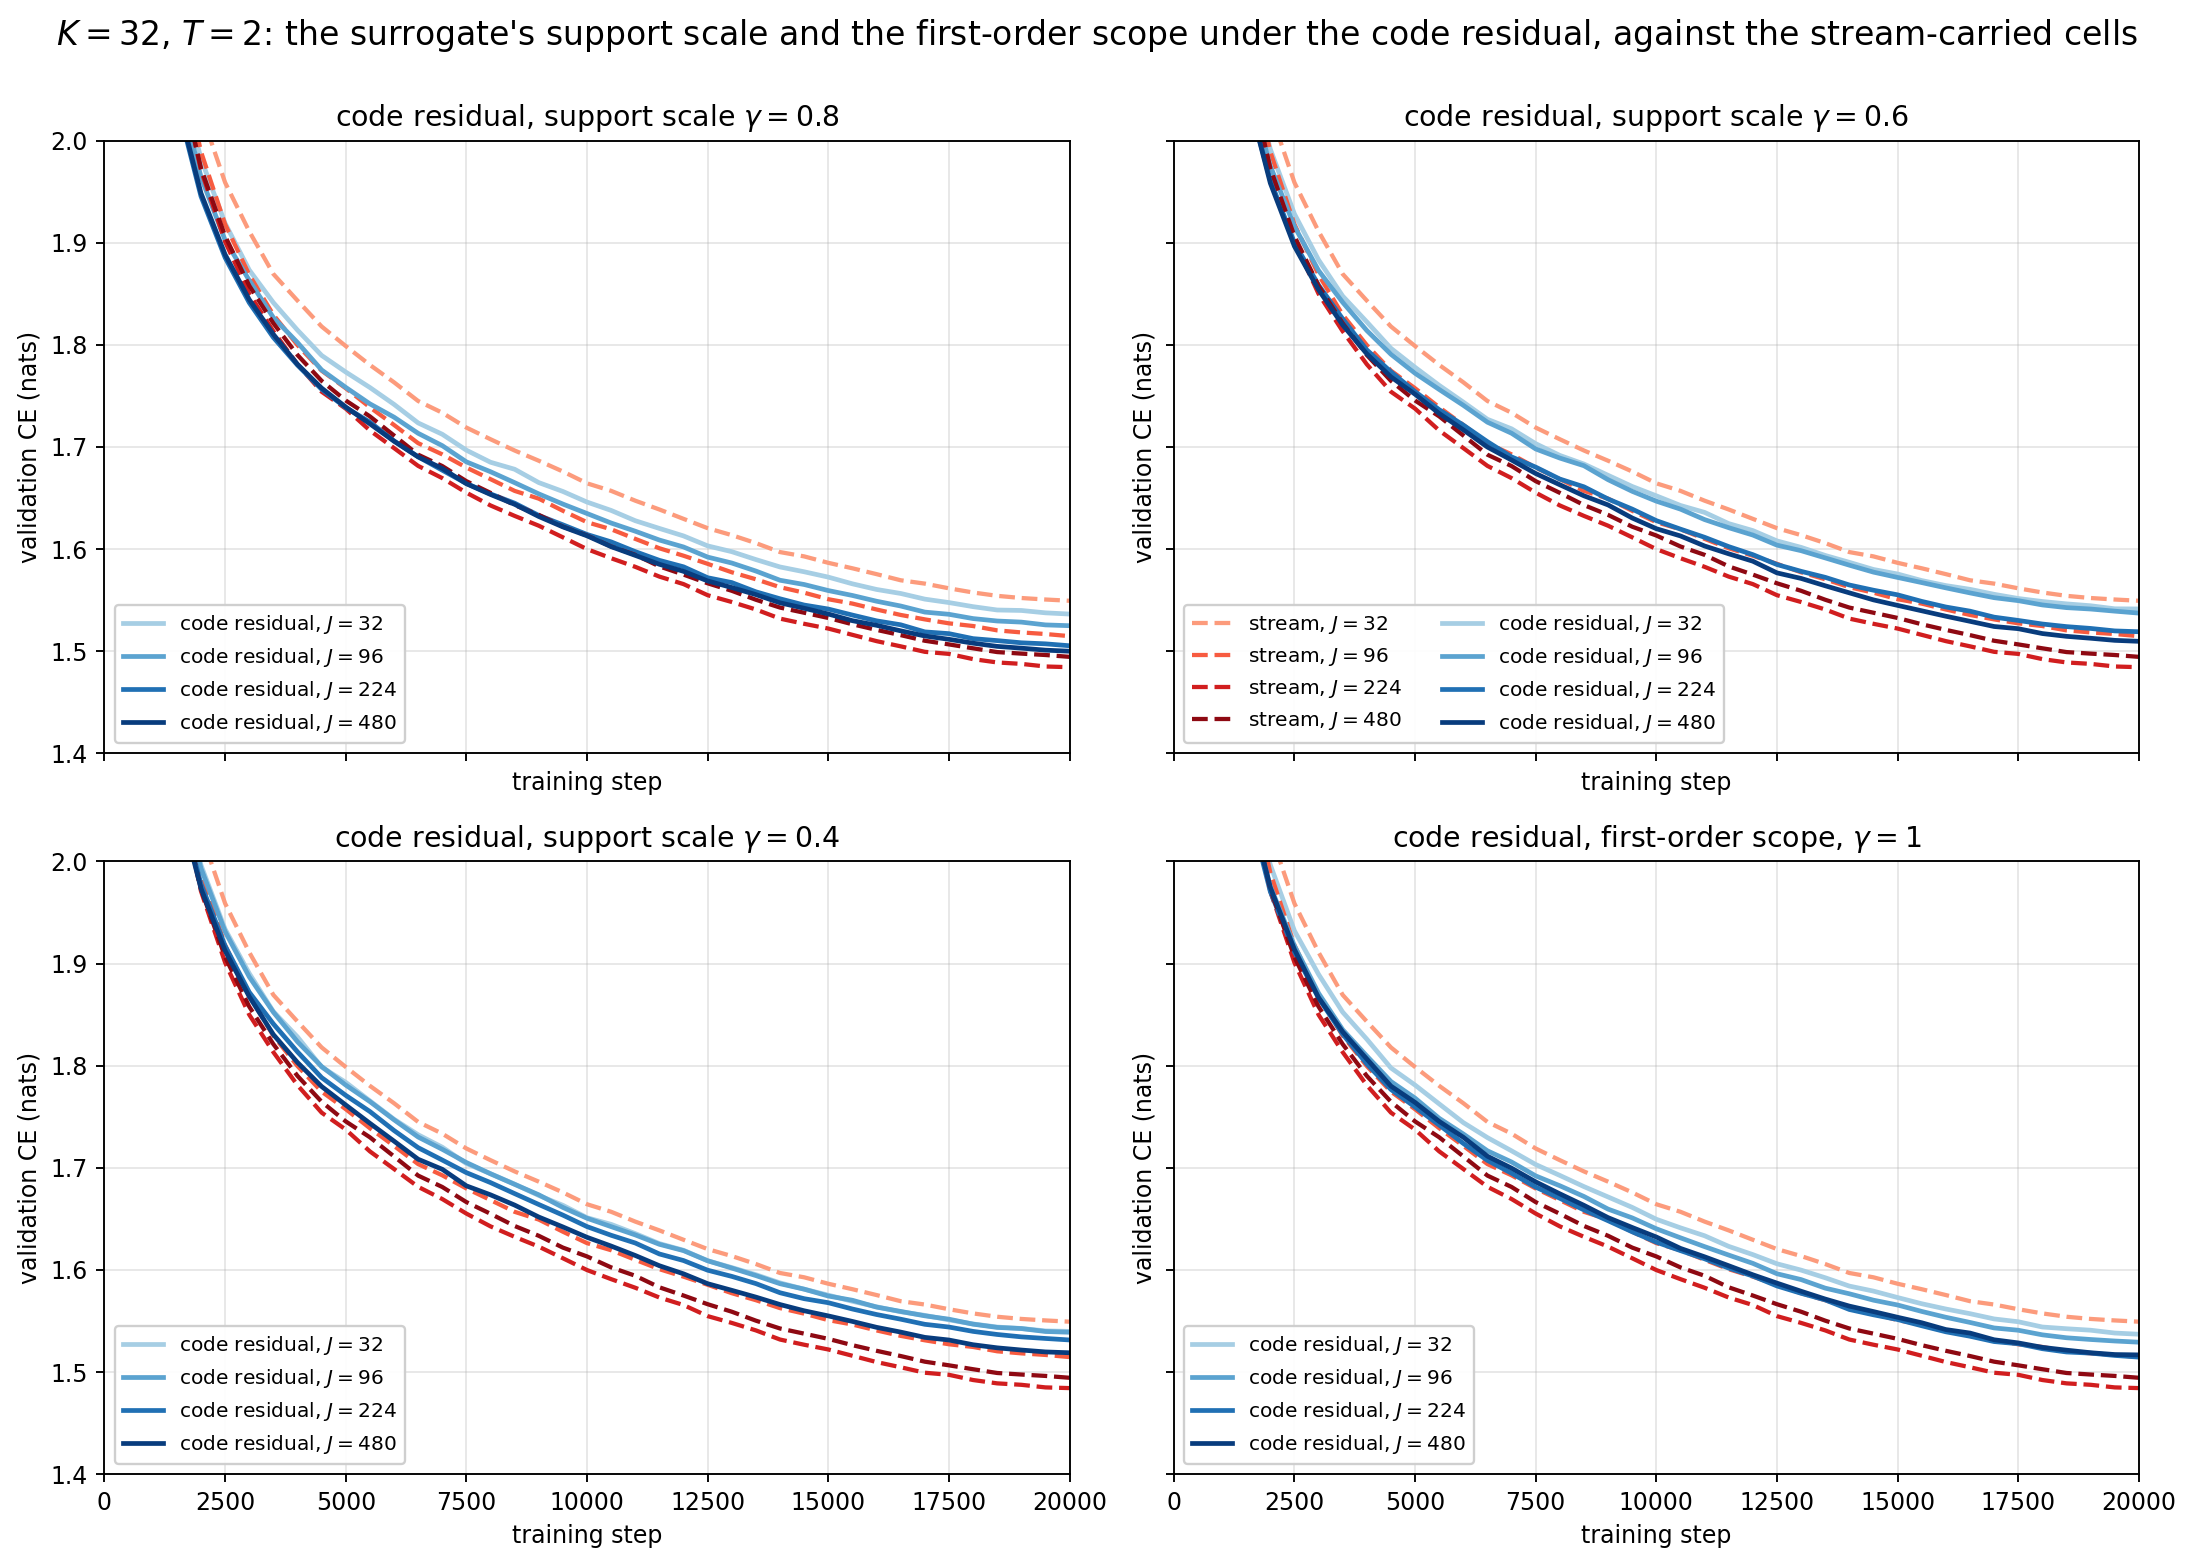
\includegraphics[width=\textwidth]{figures/kj-cr/cr_k32_sweep.png}
\caption{$K = 32$, $T = 2$, no output norm. Each panel compares one
code-carried family (solid, blue ramp light to dark with $J = 32, 96, 224,
480$) with the stream-carried $T=2$ cells at $K=32$ (dashed, red ramp):
support scale $\gamma = 0.8$, $0.6$, $0.4$, and the first-order scope at
$\gamma = 1$. In every panel the solid curve of a given $J$ runs above the
dashed one except for $J = 32$, and the gap widens from $\gamma = 0.8$ to
$\gamma = 0.4$; the first-order panel resembles the $\gamma = 0.6$ one.
Compare the $\gamma = 1$ cells in the $K = 32$ panel of the previous
section, which lie within $0.02$ of the dashed curves.}
\end{figure}

%% K=64, K=128, K=256 blocks are appended here as each K's sweep finishes
%%SWEEP-K64%%

%%SWEEP-K128%%

%%SWEEP-K256%%

% ============================================================
\section{Interpretation}
% ============================================================

Three regularities organize the grid.

First, \textbf{the carry is worth about one doubling of the active count to
a hard bottleneck, and almost nothing to the surrogate.} The hard baselines
move by $0.061$--$0.075$ nats at every $\Kp$, the ten $T=2$ surrogate cells
by $-0.012$ on average, and the margins of the K+J note shrink by the
difference: at a matched active count the surrogate's advantage over hard
Top-$K$ falls by $0.060$, $0.077$, $0.085$ and $0.073$ at $K = 32, 64, 128,
256$, which is the hard gain at that $K$ ($0.062$, $0.066$, $0.075$,
$0.065$) to within $-0.002$ to $+0.010$. The simplest reading is
that the two mechanisms supply the same thing. In the stream-carried stack
block $l{+}1$ recomputes its support from the decoded stream, and since
$E_{l+1} D_l \ne I$ a feature kept by block $l$ can be dropped at block
$l{+}1$ with $\Delta_{l+1} = 0$; gradient to the $J$ candidates lets the
encoders learn supports that survive this re-selection. The carry makes the
support persistent by construction, so the hard model receives directly what
the surrogate had to learn, and the surrogate has little left to add. The
exchange rate matches: the stream-carried surrogate bought one doubling of
$K$ (a pool of $2K$ beat hard Top-$2K$), and the code-carried hard model
lands at the stream-carried Top-$2\Kp$.

Second, \textbf{the surrogate's backward along the carry is the unstable
part.} The carry is the identity on each code coordinate, so the support
term of every gate a boundary coordinate passes multiplies its gradient by
about $1 + |u|\kappa$, with $\kappa \propto 1/T$. At $T=1$ (the post-norm
arm) this produced recurrent spikes in every cell with $K \le 128$ and five
collapses; at $T=2$ the spikes are rare and recover. The same mechanism
collapsed the 24-layer code-residual stack at $T=1$, and the $T=2$ arm here
shows that eight blocks and a kernel twice as wide keep it below the
threshold. Whether the surviving $T=2$ cells still pay for it in their final
loss is what the $K=32$ sweep of Section~6 measures: a smaller support scale
$\gamma$ or the first-order scope removes the compounding while keeping the
window.

Third, \textbf{a change that adds no parameters and no compute moved the
hard model further than the surrogate had.} The best model of the
K+J note, the $(256,256)$ post-norm surrogate at $1.4146$, is beaten by
code-carried hard Top-256 ($1.3907$) with the same active count and by
code-carried hard Top-512 ($1.3622$). For a stream bottleneck at this depth
the carry is the larger lever, and the practical default from the K+J note
-- a pool of $2K$ with the output norm -- does not transfer: under the carry
the post-norm variant is the unstable one, and the pool no longer pays for
itself against the correspondingly larger hard model.

The sweep decides between the two readings, at $T=2$: the compounding of
support terms along the carry is not what limits the code-carried surrogate
at $K=32$, since removing the products (first-order) or damping the term
($\gamma < 1$) costs rather than gains, by amounts that grow with $J$. What
the carry took from the surrogate's margin is therefore not recovered by
changing the backward; it is the re-selection that the window no longer has
to compensate, the first reading. The compounding does matter at $T = 1$,
where it collapsed half of the post-norm arm, so the two kernel widths sit
on opposite sides of its threshold at this depth. \PH{sweep at K=64, 128,
256}

% ============================================================
\section{Scope}
% ============================================================

All cells are single runs at one seed, and the two families were trained on
different GPUs; the hard-baseline differences ($0.06$--$0.075$) and the
diverged cells are far outside run-to-run variation, the surrogate
differences ($|{\Delta}| \le 0.03$) are not all so, and a seed-matched pair
of one config on the two machines would calibrate the hardware part. Five
post-norm cells did not finish, so the post-norm half of the grid has holes;
four were stopped by the divergence guard's rule (training CE more than
$2.5$ above its best for 800 steps) and one by hand after its validation CE
had reached the unigram level. The grid itself keeps the default surrogate
scope and support scale, as the single-flag premise requires; Section~6
varies both at $K=32$, $T=2$ only. The depth is eight blocks throughout,
$K + J \le 512$ well inside $N = 1536$, and the hard baselines all carry the
post-norm.

\end{document}
